\section{收敛分析}
\label{sec:ls-convergence}
\label{sec:linear-algebra-convergence-approximation}

~\ref{sec:ls-perturbation}节回答输入小变时输出变多少，本节回答另一个独立问题：
迭代、反复作用和无穷级数在步数趋于无穷时走向哪里、以多快的速度接近、
什么条件下根本不收敛。求解与逼近各章已经给出各方法的更新格式、可执行条件和
核验量，这里不重复教程，只证明误差与残差序列的极限行为：先建立有限维序列本身的
收敛判据，再分别研究固定矩阵的幂、矩阵级数与指数演化、定常迭代、Krylov迭代、
最小二乘迭代、谱方向迭代和矩阵函数迭代，最后把每步新增扰动纳入长期传播并讨论
停止精度。所有结论都在实数、有限维范围内展开；速度估计依赖具体范数和谱分布，
定性收敛与定量速度必须分开报告。

\subsection{有限维序列的收敛}
\label{sec:ls-finite-dimensional-sequences}
\label{sec:linear-algebra-sequence-convergence}

\subsubsection{收敛与误差尺度}

\paragraph{逐坐标误差与范数误差}

固定一组基$(\bm b_1,\ldots,\bm b_d)$，把向量序列$\bm x^{(t)}$写成坐标序列
$x_1^{(t)},\ldots,x_d^{(t)}$。最直接的观察方式是逐坐标比较：第$j$个坐标的误差
为$|x_j^{(t)}-x_j|$，全部坐标都随$t$趋零，等价于坐标最大范数
$\lVert\bm x^{(t)}-\bm x\rVert_c=\max_j|x_j^{(t)}-x_j|$趋零。另一种观察方式是
直接在选定范数$\lVert\cdot\rVert$下比较$\lVert\bm x^{(t)}-\bm x\rVert$。
两种方式描述的是同一个序列，但读数尺度不同：一个坐标偏差很大而其余坐标相消时，
逐坐标读数和欧氏长度可能给出不同的瞬时大小，需要先弄清二者何时互相推出。
复算小例：$\bm x^{(t)}=(1/t,\,-1/t)^{\top}$，逐坐标误差为$1/t$，欧氏长度为
$\sqrt2/t$，两者都趋零但瞬时数值相差$\sqrt2$倍；若换成斜基$\bm b_1=(1,0)$、
$\bm b_2=(1,1)$，同一向量的坐标读数又会改变，因此不能把某一种读数的大小
当作收敛速度本身。

\paragraph{两种收敛描述的等价}

~\ref{thm:ls-norm-equivalence}已经证明有限维任意两范数等价，即存在常数
$c,C>0$使$c\lVert\bm z\rVert_c\leq\lVert\bm z\rVert\leq C\lVert\bm z\rVert_c$。
于是$\lVert\bm x^{(t)}-\bm x\rVert\to0$当且仅当
$\lVert\bm x^{(t)}-\bm x\rVert_c\to0$，而后者又当且仅当每个标量坐标
$x_j^{(t)}\to x_j$。坐标收敛推出范数收敛用右端不等式，反向用左端不等式，
不需要重新证明范数等价本身。必要性方向：若范数趋零而某坐标$j$不趋零，
则$|x_j^{(t)}-x_j|$有正下界，由左端不等式$\lVert\bm x^{(t)}-\bm x\rVert\geq
c|x_j^{(t)}-x_j|$也不能趋零，矛盾。因此“序列是否收敛到某向量”与选择哪个
范数无关，后文可以按论证方便切换欧氏范数、最大范数或任意诱导范数，只在需要
定量界时才指定具体范数。边界：这一等价只在有限维成立；无限维中存在不等价
范数，坐标收敛与范数收敛可以分离，本章不涉及。

\paragraph{误差尺度变换与收敛保持}

等价常数随基和范数改变，但不改变极限本身。作固定可逆坐标变换$\bm z=\bm P\bm x$时，
有限维线性映射在任意范数下有界，故$\bm x^{(t)}\to\bm x$蕴含
$\bm P\bm x^{(t)}\to\bm P\bm x$；逆变换同样有界，反向也成立。证明：由范数等价，
$\lVert\bm P\bm x\rVert\leq C_P\lVert\bm x\rVert$，$\lVert\bm x\rVert\leq
C_{P^{-1}}\lVert\bm P\bm x\rVert$，故$\bm P$与$\bm P^{-1}$都把收敛序列映为
收敛序列。换一组范数、换一组基只重新标度误差，不创造也不消灭极限。这与
~\ref{sec:ls-norms-distances}节的尺度比较一致：定性结论（收敛、有界、闭集
保留极限）只依赖等价类，不依赖常数大小。反例边界：若变换本身随$t$变化
（例如每步换基），上述有界性不再成立，时变坐标下的极限必须单独证明，
不能沿用本段结论。

\paragraph{比较常数与速度表述}

必须把“收敛是否成立”与“以多快收敛”分开。范数等价只给出夹逼常数$c,C$，
它们用于互换存在性结论，不能当作衰减率；同一个极限在不同范数下可能第一步
放大、长期却趋零。定量速度要在具体范数下由递推结构给出，后文各节的几何因子、
谱半径和条件数才承担速度角色，本节只保证“换尺度不改变收敛与否”。例如
$\bm A=\operatorname{diag}(0.5,0.9)$在欧氏范数下每步乘缩，而取一个
非正交相似范数时前几步长度可能上升；存在性结论不变，瞬时放大却属于速度
分析。报告时应先说“是否收敛”，再在指定范数下给出几何因子或步数估计，
不得用等价常数$C$代替衰减率。

\subsubsection{极限的存在}

\paragraph{柯西条件与坐标序列}

极限未知时用柯西条件判别：对任意$\varepsilon>0$，存在$N$使$m,n>N$时
$\lVert\bm x^{(m)}-\bm x^{(n)}\rVert<\varepsilon$。由左端等价不等式，
$|x_j^{(m)}-x_j^{(n)}|\leq c^{-1}\lVert\bm x^{(m)}-\bm x^{(n)}\rVert$，
所以范数柯西列的每个坐标都是实柯西数列。实数的柯西收敛准则保证
每个坐标有实数极限$x_j$，不需要预先知道极限向量。必要性同样成立：若
某坐标不是柯西列，则存在$\varepsilon_0$与无穷多对$m,n$使
$|x_j^{(m)}-x_j^{(n)}|\geq\varepsilon_0$，由等价不等式原序列也不是
柯西列。这一步把向量柯西条件分解为$d$个标量柯西条件，标量完备性是
唯一的实数前提。

\paragraph{实数极限与向量极限的恢复}

把各坐标极限组装成$\bm x=\sum_jx_j\bm b_j$。对$m>N$，
$\lVert\bm x^{(m)}-\bm x\rVert_c=\max_j|x_j^{(m)}-x_j|$，有限个坐标的差同时
趋零，故该最大差趋零，再由右端不等式得到
$\lVert\bm x^{(m)}-\bm x\rVert\to0$。有限性在这里是关键：若坐标个数无穷，
“每个坐标趋零”不能推出最大差趋零（第$j$个坐标在$t=j$后才开始下降），
这正是无限维与有限维的分界。恢复过程只用到有限维数和标量完备性，
不依赖内积或角度。

\paragraph{有限维完备性}

结合上两段：范数柯西列逐坐标取极限、再重组为向量极限并在原范数下收敛，
所以有限维赋范空间在任意范数下都完备。这一结论不依赖欧氏结构，是范数等价的
直接推论；完备性回答“柯西列在本空间内是否有极限”，与线性空间极限的唯一性
（由三角不等式保证：若$\bm x^{(t)}\to\bm x$且$\bm x^{(t)}\to\bm y$，则
$\lVert\bm x-\bm y\rVert\leq\lVert\bm x-\bm x^{(t)}\rVert+
\lVert\bm x^{(t)}-\bm y\rVert\to0$，故$\bm x=\bm y$）是两件事。复算：
$\mathbb R^d$按任何等价范数都完备，因为它与坐标最大范数线性同构且后者
完备；不完备只发生在无限维函数空间。

\paragraph{闭子空间中的极限保留}

~\ref{thm:ls-subspace-closed}证明有限维子空间在任意范数下闭。若序列全部
落在子空间$S$内且$\bm x^{(t)}\to\bm x$，闭性保证$\bm x\in S$，不需要额外
条件。因此闭子空间本身也完备：$S$内的柯西列在全空间取到的极限必然留在$S$内。
证明：把$S$本身看作有限维赋范空间，上段完备性直接适用；全空间中取到的极限
由闭性回到$S$。求解与迭代中常用的特征空间、零空间、值域都是有限维闭子空间，
其极限分量不会逃到子空间外。边界：无限维闭子空间才需要单独证明闭性，
本章全部空间有限，可直接引用。

\paragraph{有界子列与整列收敛的区别}

闭有界集上每个序列都存在收敛子列（~\ref{sec:ls-error-scale-comparison}节的
有限维紧性），但子列存在不等于整列收敛。反例：在$\mathbb R^2$中交替取
$\bm e_1$和$-\bm e_1$，序列有界且两个子列各自常值收敛，整列却在两个点
之间振荡，不趋于任何向量；该序列甚至不是柯西列（相邻两项距离为$2$）。
再如$\bm x^{(t)}=(\sin t,0)^{\top}$，每个子列都可抽出收敛点，但整列在
$[-1,1]$上振荡。因此“抽出一个收敛子列”只能说明有界，证明整列收敛还需
柯西条件或递推给出的逐点压缩（如后文$\lVert\bm e^{(t+1)}\rVert\leq
q\lVert\bm e^{(t)}\rVert$，$q<1$）。

\subsection{矩阵连乘的长期行为}
\label{sec:ls-matrix-power-behavior}
\label{sec:linear-algebra-power-convergence}

\subsubsection{固定矩阵的幂}

\paragraph{重复作用与矩阵幂序列}

对固定方阵$\bm A$反复作用，初值$\bm x^{(0)}$在第$k$步变成
$\bm x^{(k)}=\bm A^k\bm x^{(0)}$。要判断“所有初值是否都衰减”，只检查某一个
初值的轨迹可能恰好没有经过不稳定方向，必须控制整个矩阵幂$\bm A^k$。
动机：单个初值的轨迹由初值在各特征方向上的分量决定，若初值碰巧不含某个
$|\lambda|\geq1$方向，轨迹看起来收敛，换一个初值立即发散。全体初值收敛等价于
$\bm A^k\to\bm0$（矩阵序列在诱导范数下趋零），这比“存在某个收敛初值”强得多。
下面先给全体初值的衰减判据，再处理$\rho(\bm A)=1$边界上的有界、振荡与增长。

\paragraph{次乘性与实幂增长率}

诱导范数次乘性给出$\lVert\bm A^{k+\ell}\rVert\leq\lVert\bm A^k\rVert
\lVert\bm A^\ell\rVert$，特别地$\lVert\bm A^k\rVert\leq\lVert\bm A\rVert^k$。
若$\lVert\bm A\rVert<1$，则$\lVert\bm A^k\rVert\leq\lVert\bm A\rVert^k\to0$，
这是一条可直接核验的充分条件；但它不是必要条件，因为范数可以通过非正交方向的
相消把瞬时长度放大，长期却由谱决定。复算：$\bm A=\operatorname{diag}(0.5,0.9)$
在任意范数下都有$\rho=0.9<1$，但在某个斜置等价范数中$\lVert\bm A\rVert$可
大于$1$，充分条件失效而衰减仍然成立。次乘性也给出有界性：$\lVert\bm A\rVert\leq1$
只保证$\lVert\bm A^k\rVert$不超过$\lVert\bm A\rVert^k\leq1$，不保证趋零；
等号情形（如$\bm A$为正交旋转）长度恒定，需逐类判别。

\paragraph{分块幂估计与几何上界}

由实Schur或实分裂的Jordan分块表示（见下一小节），每个块的幂都是有限次多项式
乘以模长$r^k$。对任意$r>\rho(\bm A)$，多项式增长$k^s$总能被较大的几何因子
$r^k$控制，因为$\lim_{k\to\infty}k^s/r^k=0$，故存在常数$C_r$使
$\lVert\bm A^k\rVert\leq C_r r^k$。证明要点：每个特征值$\lambda_i$满足
$|\lambda_i|<r$，有限个块各自有界，换基矩阵固定，合并即得。这一估计把
“谱半径小于某数”翻译成可用于递推的几何上界，常数$C_r$依赖矩阵和$r$，
随$r\downarrow\rho(\bm A)$可能增大；当$\rho(\bm A)=0$（幂零矩阵）时
$\bm A^s=\bm0$，有限步后恰为零，比几何衰减更快。

\paragraph{谱半径和所有初值的衰减}

\begin{theorem}[固定矩阵幂的衰减判据]
\label{thm:ls-power-decay}
对有限实方阵$\bm A$，$\bm A^k\to\bm0$当且仅当谱半径
$\rho(\bm A)=\max_i|\lambda_i(\bm A)|<1$。
\end{theorem}
\begin{proof}
必要性：若$\bm A^k\to\bm0$，对任一实特征向量$\bm v$与特征值$\lambda$，
$\bm A^k\bm v=\lambda^k\bm v\to\bm0$，故$|\lambda|<1$；非实共轭对在实二维
块中以模$|\lambda|$旋转衰减，同样要求$|\lambda|<1$。若存在$|\lambda|\geq1$，
取该方向（或共轭对张成的实平面）内任一初值，$\lVert\bm A^k\bm x\rVert$不趋零，
与全体初值衰减矛盾。充分性：取$r$满足$\rho(\bm A)<r<1$，由分块估计
$\lVert\bm A^k\rVert\leq C_r r^k\to0$，有限块合并后仍趋零。零特征值块在
有限步后恰为零。
\end{proof}
该判据针对全体初值：只要存在模不小于$1$的特征值，对应方向的误差就不能趋零。
注意判据是充要条件，而非仅充分；$\lVert\bm A\rVert<1$只是充分的可核验手段。

\paragraph{固定点空间与剩余方向}

把特征值按模长分组：$|\lambda|<1$的方向随$k$衰减，$|\lambda|=1$的方向保持长度
（实特征值$\lambda=1$固定不动，$\lambda=-1$反向振荡，非实共轭对旋转），
$|\lambda|>1$的方向增长。全体初值的长期行为由单位模方向决定，衰减方向只留下
有限步的瞬态贡献。复算：$\bm A=\operatorname{diag}(0.5,1,2)$，初值
$\bm x^{(0)}=(a,b,c)^{\top}$的第二分量$b$恒定、第三分量$c\cdot2^k$发散、
第一分量$a\cdot0.5^k$趋零；只要$c\neq0$整列发散，与前两个分量无关。
这说明“矩阵有衰减方向”不能推出“全体初值收敛”。

\paragraph{非零有限极限与投影}

$\bm A^k$有有限极限当且仅当所有特征值位于开单位圆内，或等于$1$且属于$1$的
Jordan块全为$1\times1$（没有幂零耦合）。此时极限把向量投影到$\lambda=1$的
特征空间，其余分量被抹去。例如$\operatorname{diag}(1,0.5)^k$保留第一坐标、
衰减第二坐标，收敛到该投影，而不是零矩阵。边界：若$\lambda=1$出现在
$s\geq2$的Jordan块中，块幂含$(k-1)\bm N$项，$\bm A^k$无有限极限；
$\lambda=-1$的块即使对角化也使$\bm A^k$在两个矩阵间交替，不取单一极限；
$|\lambda|>1$或$|\lambda|=1$的非实共轭对均不收敛到固定矩阵。

\paragraph{单位边界的有界、振荡和增长}

$\rho(\bm A)=1$必须逐类判别，不能由“谱半径等于1”统一推出结论：
$\operatorname{diag}(-1,0.5)^k$通常振荡不收敛到固定矩阵；
$\begin{smallmatrix}1&1\\0&1\end{smallmatrix}^k=\begin{smallmatrix}1&k\\0&1\end{smallmatrix}$
含线性增长的$k$项而无界；$\operatorname{diag}(1,0.5)^k$收敛到投影；
$|\lambda|>1$时至少有初值发散，但不代表每个初值都发散（不含该方向的初值
仍可收敛）。四类边界（固定投影、交替振荡、多项式增长、几何增长）对应
不同特征值结构，必须先求谱再下结论。

下面的固定例把短时放大与长期衰减放在同一条轨迹上。取
$\bm A=\begin{bmatrix}0.8&4\\0&0.5\end{bmatrix}$、
$\bm x^{(0)}=(0,1)^{\top}$，每步作用一次：
\begin{equation}
 \bm A=\begin{bmatrix}0.8&4\\0&0.5\end{bmatrix},\qquad
 \bm x^{(k+1)}=\bm A\bm x^{(k)}.
 \label{eq:ch06-fixed-iteration-example}
\end{equation}
第一步$\bm x^{(1)}=(4,0.5)^{\top}$已比初值长得多，$\lVert\bm A\rVert_2>4$，
但$\rho(\bm A)=0.8$，长期逐项趋零。图~\ref{fig:ch06-transient-growth}把同一
迭代的轨迹和长度并列，显示短时放大与长期衰减并不矛盾：特征值决定长期，
非正交特征方向间的相消决定早期长度。

\begin{figure*}[htbp]
  \centering
  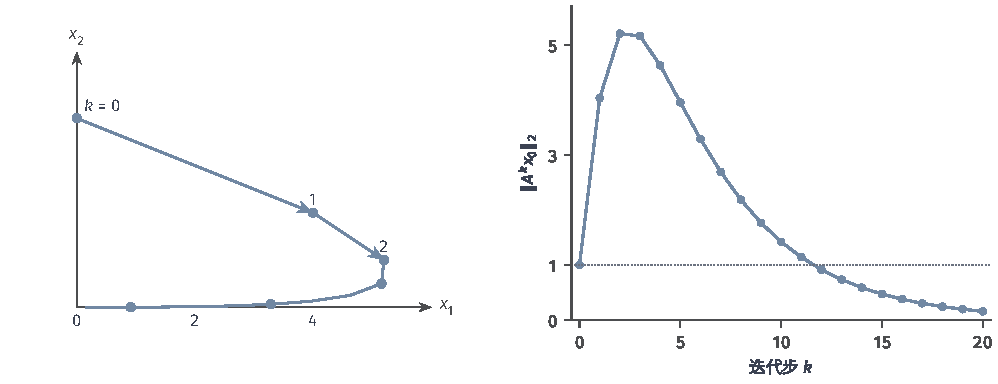
\includegraphics[width=169.0mm]{figures/01-mathematical-preliminaries-upper/02-linear-spaces/matplotlib/ch06-transient-growth/figure.pdf}
  \caption{固定二维矩阵的反复作用。初值为$(0,1)^{\top}$，前两步的长度增加，
  此后回到原点；右图将长度与初始长度$1$比较。特征值$0.8$和$0.5$决定长期衰减，
  非正交特征方向间的相消则决定早期放大。两图使用同一个矩阵和同一组迭代点。}
  \label{fig:ch06-transient-growth}
\end{figure*}

该矩阵可对角化，特征向量$\bm v_1=(1,0)^{\top}$、$\bm v_2=(-40/3,1)^{\top}$
对应$0.8$和$0.5$，因而
\begin{equation}
 \bm A^k=
 \begin{bmatrix}
  0.8^k&\frac{40}{3}(0.8^k-0.5^k)\\
  0&0.5^k
 \end{bmatrix},\qquad
 \bm x^{(k)}=
 \begin{bmatrix}\frac{40}{3}(0.8^k-0.5^k)\\0.5^k\end{bmatrix}.
 \label{eq:ch06-diagonalizable-finite-trajectory}
\end{equation}
$k=1,2,3$分别给$(4,0.5)^{\top}$、$(5.2,0.25)^{\top}$、$(5.16,0.125)^{\top}$，
与逐步相乘一致。初值实际写成$\tfrac{40}{3}\bm v_1+\bm v_2$，两个大横向分量
初始相消；衰减速度不同使相消被打破，长度先增大后回落。

\subsubsection{谱结构与增长速度}

\paragraph{特征方向不足与广义特征链}

当几何重数小于代数重数时，独立特征向量张不满空间，需要广义特征向量补齐：
对正整数$j$满足$(\bm A-\lambda\bm I)^j\bm v=\bm0$的非零向量。一条链从特征
向量$\bm v_1$开始，后续满足$(\bm A-\lambda\bm I)\bm v_{j+1}=\bm v_j$，
减去共同缩放后每个方向被送到链中前一个方向。动机：仅有的几个特征方向无法
分解任意初值，而幂$\bm A^k$沿链逐级平移，必须知道链长才能解释多项式增长。
复算：$\bm J=\begin{smallmatrix}0.8&1\\0&0.8\end{smallmatrix}$只有一个
特征向量$(1,0)^{\top}$，初值$(0,1)^{\top}$不在其中，若只按特征方向分解
就会漏掉第二坐标的耦合项。

\paragraph{实分裂条件下的Jordan块}

本节只处理特征多项式实分裂的情形（全部特征值为实数），非实共轭对留给实Schur块。
在链基下矩阵由块$\bm J_s(\lambda)=\lambda\bm I+\bm N$组成，$\bm N$为
$s\times s$幂零矩阵、$\bm N^s=\bm0$，超对角元为$1$。相似变换
$\bm J_s=\bm P^{-1}\bm A\bm P$保持谱与幂的长期行为（$\bm A^k=
\bm P\bm J_s^k\bm P^{-1}$），所以块分析可直接用于原矩阵。这是相似分类的
标准形，用于解释结构，数值计算通常不主动构造对扰动极敏感的链基。

\paragraph{链长度与相似分类}

块大小$s$等于该$\lambda$对应的最长链长度，即代数重数减去几何重数后的耦合深度。
$s=1$是普通特征方向；$s>1$记录“缺少独立特征方向”。例如
$\begin{smallmatrix}0.8&1\\0&0.8\end{smallmatrix}$只有一个特征方向，
不能因为对角元相同就当作$0.8\bm I$：后者可对角化、幂直接是$0.8^k\bm I$，
前者幂含$k0.8^{k-1}$耦合项，长期速度虽同为指数衰减，有限步轨迹不同。
判别方法：解$(\bm A-0.8\bm I)\bm v=0$只得到一维解空间，几何重数为$1$、
代数重数为$2$，故必有$s=2$块。

\paragraph{块幂中的多项式增长因子}

对$\bm J=\lambda\bm I+\bm N$作二项式展开（$\lambda\bm I$与$\bm N$可交换），
\begin{equation}
 \bm J^k=\sum_{j=0}^{\min(k,s-1)}\binom{k}{j}\lambda^{k-j}\bm N^j,
 \qquad k=0,1,\ldots.
 \label{eq:ch06-jordan-power}
\end{equation}
$\lambda=0$时$\bm J^k=\bm N^k$，$k\geq s$后恰为零（幂零）；$\lambda\neq0$时
$\binom{k}{j}$提供至多$s-1$次的多项式因子，而整体仍带$\lambda^k$指数。以
$\bm J=\begin{bmatrix}0.8&1\\0&0.8\end{bmatrix}$为例，
$\bm J^k=\begin{bmatrix}0.8^k&k\,0.8^{k-1}\\0&0.8^k\end{bmatrix}$，
初值$(0,1)^{\top}$第一步成为$(1,0.8)^{\top}$、第二步成为$(1.6,0.64)^{\top}$；
第一坐标的累积项$k0.8^{k-1}$先上升（$k\approx5$附近达到约$2.05$）再由指数
衰减主导。图~\ref{fig:vol1-add-linear-jordan-accumulation}画出两个坐标的
逐步变化。边界：多项式因子永远压不过$|\lambda|^k$，所以$\rho<1$时块幂
仍趋零，只是比对角情形慢一个多项式阶；$\rho=1$且$\lambda=1$的$s>1$块则
线性发散。

\begin{figure}[!htb]
  \centering
  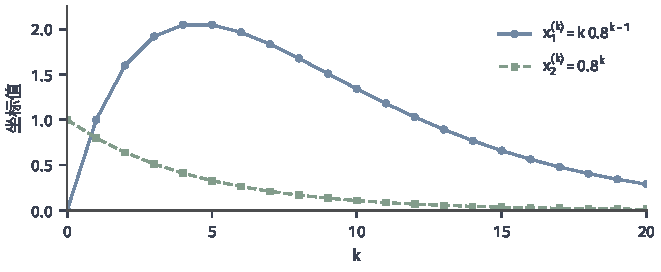
\includegraphics[width=112mm]{figures/01-mathematical-preliminaries-upper/02-linear-spaces/matplotlib/comprehension-additions/linear-jordan-accumulation.pdf}
  \caption{Jordan块的累积项。取正文$\bm J=\left[\begin{smallmatrix}0.8&1\\0&0.8\end{smallmatrix}\right]$与初值$(0,1)^{\top}$。绿线为$0.8^k$，蓝线在$k\geq1$时为$k0.8^{k-1}$，在$k=0$时为$0$。点表示整数步，连线仅引导读图；两坐标最终都趋零。}
  \label{fig:vol1-add-linear-jordan-accumulation}
\end{figure}

若$\bm A=\bm V\bm\Lambda\bm V^{-1}$实可对角化，对定义在其谱上的单值函数$f$，
\begin{equation}
 f(\bm A)=\bm V\operatorname{diag}(f(\lambda_1),\ldots,f(\lambda_d))\bm V^{-1}.
 \label{eq:matrix-analysis-matrix-function-diagonalizable}
\end{equation}
不可对角化时仅给根上的函数值不够，还要块大小所需的导数：
\begin{equation}
 f(\bm J_s(\lambda))=\sum_{j=0}^{s-1}\frac{f^{(j)}(\lambda)}{j!}\bm N^j,
 \label{eq:ch06-jordan-function}
\end{equation}
这是Taylor展开在$\bm N^s=\bm0$后精确终止的结果。证明：把$f$在$\lambda$处
展开，$(\bm J_s-\lambda\bm I)=\bm N$，高阶项$\bm N^j$在$j\geq s$为零，
逐项代入即得。函数中的多项式因子$t^j/j!$不是数值近似误差，而是幂零耦合的
真实作用；$f$在$\lambda$处不可导时，Jordan块上的$f(\bm A)$无法良好定义。

\paragraph{实Schur块与旋转衰减}

一般实矩阵取实Schur形式，$\bm Q$正交，$\bm T$为分块上三角，对角块大小为
$1$或$2$：
\begin{equation}
 \bm A=\bm Q\bm T\bm Q^{\top},\qquad \bm Q^{\top}\bm Q=\bm I.
 \label{eq:matrix-analysis-schur-decomposition}
\end{equation}
$2\times2$块对应非实共轭特征值对，形如
$\begin{bmatrix}a&-b\\b&a\end{bmatrix}=r\!\begin{bmatrix}\cos\theta&-\sin\theta\\\sin\theta&\cos\theta\end{bmatrix}$，
其幂为$r^k$乘旋转$k\theta$，$r=\sqrt{a^2+b^2}=|\lambda|$；
$r<1$时旋转振荡地衰减，$r=1$时在圆周上匀速旋转不取极限，$r>1$时增长。
上三角耦合项在块稳定时被几何因子吸收：把块按$r^k$归一，耦合贡献含额外
$r^k$因子，长期可忽略。

\paragraph{特征基条件与瞬态放大}

可对角化但非正交时，
\[
\lVert\bm A^k\rVert_2\leq
\lVert\bm V\rVert_2\lVert\bm V^{-1}\rVert_2\max_i|\lambda_i|^k,
\]
坐标放大因子$\lVert\bm V\rVert\lVert\bm V^{-1}\rVert$进入有限步界，它只在
$k$大时被$\max|\lambda_i|^k$压过，早期不受谱控制。自伴情形$\bm V$可取
正交，该因子为$1$；非正交基不能忽略它，这正是上面二维例短时放大的来源。
边界：该界是上界，非正交基病态时实际早期长度可能更大，但长期衰减率仍由
$\rho$决定，二者不矛盾。

\paragraph{分析表示和数值表示的区别}

Jordan形式用于解释结构和证明速度，微小扰动就可能改变块结构（把一个$s=2$块
拆成两个近邻特征值），数值识别精确块并不稳健；实际计算采用Schur形式只处理
稳定的分块上三角，不主动构造链基。分析结论（$\rho<1$趋零）与数值实现
（避免病态基）分工明确：证明用Jordan链说明多项式因子，工程计算用Schur块
避免对扰动敏感的基变换。

\subsubsection{非负矩阵的反复作用}

\paragraph{非负作用与质量传递}

逐项非负的$\bm A\geq0$（每个元素$a_{i,j}\geq0$）把非负向量$\bm x\geq0$映为
非负向量$\bm A\bm x\geq0$，分量之间只转移不创造。把$\bm x$看作各通道的质量，
$(\bm A\bm x)_i=\sum_j a_{i,j}x_j$是从$j$流入$i$的总量，$\bm A^k\bm x$描述
经过$k$步传递后的分布。非负性使各分量不会因相消变号，因而可以用分量比值
（而非范数）刻画方向收敛，这是Perron理论比一般谱分析更精细的原因。本小节只做
代数的收敛分析，概率转移的随机解释留待概率卷。

\paragraph{正矩阵的比值极值与正特征方向}

正矩阵（所有元素严格为正）满足Perron--Frobenius理论的最干净情形：谱半径
$\rho(\bm A)$本身是一个正特征值，对应一个严格为正的特征向量，且模不超过
$\rho(\bm A)$的其他特征值都不可能与之并列主导\scite{math-horn2013matrix}。
Collatz--Wielandt比值检验给出存在性与上下界：对任意正向量$\bm x>0$取
$m(\bm x)=\min_i(\bm A\bm x)_i/x_i$与$M(\bm x)=\max_i(\bm A\bm x)_i/x_i$，
则$m(\bm x)\leq\rho(\bm A)\leq M(\bm x)$。证明要点：设$\bm p>0$为Perron
方向、$\bm A\bm p=\rho\bm p$，令$s=\min_i x_i/p_i$、$t=\max_i x_i/p_i$，
则$\bm x\geq s\bm p$、$\bm x\leq t\bm p$，由非负性$\bm A\bm x\geq s\rho\bm p$
给出$m(\bm x)\geq s\rho$，$\bm A\bm x\leq t\rho\bm p$给出$M(\bm x)\leq t\rho$，
两式相除并取遍分量即得夹逼。复算正矩阵$\bm P=\begin{smallmatrix}1&2\\3&4\end{smallmatrix}$，
$\rho(\bm P)=(5+\sqrt{33})/2\approx5.3723$；取正向量$\bm x=(1,1)^{\top}$，
$\bm P\bm x=(3,7)^{\top}$，比值$m=3\leq5.3723\leq M=7$。再作用一次
$\bm P^2\bm x=(17,37)^{\top}$，比值区间收紧到$[5.286,5.667]$，第三步
$[5.353,5.378]$，逐次夹到$\rho$，演示区间单调收紧。反复作用$\bm A^k\bm x$时比值区间
$[m(\bm A^k\bm x),M(\bm A^k\bm x)]$单调收紧到$\rho(\bm A)$。
适用条件：$\bm A$不可约（本原矩阵更直接）且初值$\bm x>0$为正向量；
证明收紧方向：每作用一次，比值区间被夹逼关系重新包裹，$s,t$随$\bm A^k\bm x$
趋于Perron方向而收敛到同一比值，故区间两端收敛到$\rho$。边界：可约矩阵或
初值在某对角块上投影为零时，区间可能卡在该块的Perron根而不收紧到整矩阵的
$\rho$，不能把夹逼结论无条件外推。

\paragraph{非负逼近与不可约条件}

元素含零的非负矩阵要先区分连通性：把下标看作有向图的顶点，$a_{i,j}>0$即从$j$到$i$
有边，\term{不可约}（irreducible）指该图强连通，任意两顶点间有正向路径。
可约矩阵可经置换写成块上三角，各对角块独立传递，整矩阵的主方向由各块比较决定，
不能直接套用正矩阵结论。复算：$\bm A=\operatorname{diag}(0.5,0.8)$可约，
两个块各有自己的Perron根，长期方向由较大的$0.8$块决定，另一块分量直接衰减，
不存在全体正的公共主方向。

\paragraph{Perron根与主方向的尺度}

不可约非负矩阵仍有$\rho(\bm A)>0$作为一个单特征值（代数重数为$1$），对应
严格正的Perron方向$\bm p>0$；但其他特征值可以具有同一模$|\lambda|=\rho(\bm A)$，
此时长期行为不是单一方向。$\bm p$只在相差一个正倍数的意义下确定，归一化
（除以分量和或长度）去掉任意尺度。条件要点：上述正Perron方向与单重性要求
不可约；可约矩阵的Perron根可能多重，且主方向只在主导块内为正。

\paragraph{正幂下的收缩与归一化极限}

不可约且\term{本原}（primitive），即存在$k_0$使$\bm A^{k_0}>0$（某一幂把所有
零位置填正），则其余特征值的模都严格小于$\rho(\bm A)$。于是对任意非零
$\bm x\geq0$，归一化幂序列
$\bm A^k\bm x/\lVert\bm A^k\bm x\rVert$收敛到Perron方向；未归一化时
$\bm A^k\bm x$按$\rho(\bm A)^k$增长或衰减，方向先于尺度稳定。证明要点：
把$\bm x$在特征基展开，主导项为$\rho^k c\bm p$，其余项按$|\lambda_j|^k$
（$|\lambda_j|<\rho$）衰减，除以$\rho^k$后余项趋零，方向趋于$\bm p$。
初值条件：$\bm x\geq0$且不含零分量在主导块上的投影为零；本原性保证
$\bm A^{k_0}>0$把任何非零非负初值都变成正向量，故初值限制很弱。

\paragraph{周期情形的振荡边界}

不可约但非本原的矩阵有周期$p>1$：存在$p$个模同为$\rho(\bm A)$的特征值，
均匀分布在半径$\rho(\bm A)$的圆周上（实矩阵中成共轭对出现）。归一化序列在$p$个
循环类之间轮换，$k$模$p$不同时落在不同方向，不存在单一极限；这是
$\rho(\bm A)=1$边界振荡在非负矩阵中的具体形态。复算：$p=2$的置换矩阵
$\begin{smallmatrix}0&1\\1&0\end{smallmatrix}$，$\bm A^k$在$\bm I$与$\bm A$间
交替，归一化方向轮换，永不收敛到固定向量。

\paragraph{随机矩阵的代数保持与概率入口}

行和（或列和）全为$1$的非负矩阵称为\term{随机矩阵}（stochastic matrix），
代数上它保持总质量：$\sum_i(\bm A\bm x)_i=\sum_jx_j$（行和口径，因为
$\sum_i a_{i,j}=1$），$\rho(\bm A)=1$且$1$为特征值。本原随机矩阵的归一化
分布收敛到平稳Perron方向，这里只用到质量保持与方向收敛；“分布收敛到平稳分布”
的概率论证（遍历性、期望收敛）属于概率卷，这里不展开。边界：可约随机矩阵
存在多个闭类，初值落在哪个闭类就收敛到哪个平稳分布，不存在全体初值的公共极限。

\subsubsection{变化矩阵的连乘}

\paragraph{变化矩阵与有序乘积}

迭代中每步矩阵可能不同，第 $k$ 步乘积写成 $\bm B_k\cdots\bm B_1\bm x^{(0)}$，
误差按同一顺序累积。与固定矩阵不同，每一步的谱半径都小于$1$并不能保证乘积
衰减，因为各步作用的方向不一致：$\rho(\bm B_j)<1$只描述$\bm B_j$自身的
长期行为，而乘积的早期放大由各步方向间的夹角决定，谱半径不携带这一信息；
必须用乘积整体控制，不能逐步检查谱半径。

\paragraph{逐步谱半径不足的例子}

取$\bm B_1=\begin{bmatrix}0&2\\0&0\end{bmatrix}$、
$\bm B_2=\begin{bmatrix}0&0\\2&0\end{bmatrix}$，二者$\rho=0$且都是幂零的，
但$\bm B_2\bm B_1=\operatorname{diag}(0,4)$把第二分量放大$4$倍。
逐步相乘复算：$\bm B_1$把$(x_1,x_2)^{\top}$映为$(2x_2,0)^{\top}$，
$\bm B_2$再映为$(0,2\cdot2x_2)^{\top}=(0,4x_2)^{\top}$。
单个矩阵没有非零谱，两步交换方向后却产生放大，说明必须用乘积整体控制，
不能逐步检查谱半径。

\paragraph{共同范数与一致收缩}

若存在同一个范数使所有$\lVert\bm B_k\rVert\leq q<1$（一致收缩），则
$\lVert\bm B_k\cdots\bm B_1\rVert\leq q^k$，任意初值误差按几何因子$q^k$衰减。
关键是“同一个范数、同一个上界”；每步换范数或上界随$k$接近$1$，结论都不成立。
证明由次乘性归纳：$\lVert\bm B_k\cdots\bm B_1\rVert\leq
\lVert\bm B_k\rVert\lVert\bm B_{k-1}\cdots\bm B_1\rVert\leq q\cdot q^{k-1}$。

\paragraph{连乘界与初值误差衰减}

由次乘性递推，
$\lVert\bm e^{(k)}\rVert\leq\lVert\bm B_k\rVert\cdots\lVert\bm B_1\rVert
\lVert\bm e^{(0)}\rVert$。一致收缩时该乘积$\leq q^k\lVert\bm e^{(0)}\rVert$，
初始误差被整体压小，不需要逐坐标跟踪。边界：若仅$\lVert\bm B_k\rVert\leq1$
而无统一$q<1$，只能得到有界，不能推出趋零；若各步上界$q_k\to1$，乘积
$\prod q_k$可能不趋零。

\paragraph{作用顺序与累计放大}

矩阵不可交换，顺序不能随意调换：上例中$\bm B_1\bm B_2=\operatorname{diag}(4,0)$
放大的是第一分量。复算：$\bm B_2$先把$(x_1,x_2)^{\top}$映为$(0,2x_1)^{\top}$，
$\bm B_1$再映为$(2\cdot2x_1,0)^{\top}=(4x_1,0)^{\top}$。连乘界按实际作用
顺序相乘，重排步序会改变放大方向，比较两种实现时必须保留各自顺序。

\paragraph{缺少共同控制时的边界}

不存在共同一致收缩界时，乘积可能在某段内放大，是否长期收敛需要联合结构
（共同不变度量、联合谱半径等），超出本卷范围；本卷只要求识别“逐步谱半径小”
不是充分条件这一边界，不为变化矩阵编造统一衰减保证。

\subsection{矩阵级数与指数演化}
\label{sec:ls-matrix-series-exponential}

\subsubsection{矩阵级数}

\paragraph{部分和与尾项误差}

矩阵幂级数$\sum_{k=0}^{\infty}\bm A^k$的第$N$部分和
$\bm S_N=\sum_{k=0}^N\bm A^k$；级数收敛指$\bm S_N$作为矩阵序列收敛。
尾项$\sum_{k>N}\bm A^k$就是部分和与极限的差距，需要可计算的尾界而不是
只看通项趋零。动机：通项$\bm A^k\to0$只是级数收敛的必要条件，标量级数
$\sum 1/k$通项趋零却发散，矩阵级数同样不能仅凭通项判断；截断到$N$步时
必须给出尾项范数上界才能报告近似精度。

\paragraph{幂衰减下的Neumann收敛}

\term{Neumann级数}（Neumann series）$\sum_{k=0}^{\infty}\bm A^k$在
$\lVert\bm A\rVert<1$（某次乘性范数）时收敛。这是绝对收敛：
$\sum_k\lVert\bm A^k\rVert\leq\sum_k\lVert\bm A\rVert^k<\infty$，
由有限维范数等价保证矩阵级数绝对收敛即收敛。证明：绝对收敛的矩阵级数其
每个元素都是绝对收敛的标量级数，有限个元素同时收敛，故部分和矩阵收敛。

\paragraph{部分和恒等式与逆的构造}

逐项相消恒等式
$(\bm I-\bm A)\sum_{k=0}^N\bm A^k=\bm I-\bm A^{N+1}$，直接展开左侧：
$\sum_{k=0}^N\bm A^k-\sum_{k=1}^{N+1}\bm A^k=\bm I-\bm A^{N+1}$。
$\lVert\bm A\rVert<1$时$\bm A^{N+1}\to\bm0$，令$N\to\infty$得
$(\bm I-\bm A)\sum_{k=0}^{\infty}\bm A^k=\bm I$，故$\bm I-\bm A$可逆且
\begin{equation}
 (\bm I-\bm A)^{-1}=\sum_{k=0}^{\infty}\bm A^k.
 \label{eq:ls-neumann-series}
\end{equation}
右侧同样给出$(\sum\bm A^k)(\bm I-\bm A)=\bm I$，左逆即右逆。这是用级数
构造逆的显式公式，也给出逆的存在性充分条件；复算标量$\bm A=0.5$时
$(1-0.5)^{-1}=2=1+0.5+0.25+\cdots$，与几何级数一致。

\paragraph{几何尾界的范数条件}

尾项满足
$\lVert\sum_{k>N}\bm A^k\rVert\leq
\sum_{k>N}\lVert\bm A\rVert^k=
\lVert\bm A\rVert^{N+1}/(1-\lVert\bm A\rVert)$，
可直接用于截断误差估计。条件写为$\lVert\bm A\rVert<1$是充分的；
谱半径$\rho(\bm A)<1$时由~\ref{sec:ls-matrix-power-behavior}节分块估计仍可收敛，
但要先换到一个使范数上界小于$1$的等价范数，不能直接使用原范数尾界。
边界：$\lVert\bm A\rVert=1$时几何尾界分母为零，给不出衰减；$\rho(\bm A)<1$
而原范数$\geq1$时级数仍收敛，只是尾界需换范数后重算。

\paragraph{一般幂级数的收敛范围}

对标量幂级数$f(s)=\sum_{k=0}^{\infty}a_ks^k$的收敛半径$R$，矩阵级数
$\sum_{k=0}^{\infty}a_k\bm A^k$在$\rho(\bm A)<R$时收敛；$\rho(\bm A)>R$
发散，$\rho(\bm A)=R$边界上逐项判断。Jordan块中的多项式因子被$R^{-k}$吸收，
不改变收敛半径。复算：$f(s)=1/(1-s)$的$R=1$，对应Neumann级数；
$f(s)=e^s$的$R=\infty$，所以矩阵指数对任意$\bm A$收敛。

\paragraph{离散Lyapunov级数的构造}

离散时间稳定传播$\bm x^{(t+1)}=\bm A\bm x^{(t)}$下，正定Gram量
$\bm P=\sum_{k=0}^{\infty}(\bm A^{\top})^k\bm Q\bm A^k$（$\bm Q\succeq0$）
是离散Lyapunov方程
$\bm P-\bm A^{\top}\bm P\bm A=\bm Q$的解。把级数代入：
$\bm P-\bm A^{\top}\bm P\bm A=\bm Q+\sum_{k\geq1}(\bm A^{\top})^k\bm Q\bm A^k-
\sum_{k\geq0}(\bm A^{\top})^{k+1}\bm Q\bm A^{k+1}=\bm Q$，逐项相消。
级数收敛的条件正是$\rho(\bm A)<1$，每一项按$\rho^{2k}$量级衰减，级数
才有意义；该级数也是误差协方差在稳定传播下的长期累积。

\paragraph{正定性、唯一性与稳定条件}

$\bm Q\succ0$且$\bm A$稳定时$\bm P\succ0$：对任意非零$\bm x$，
$\bm x^{\top}\bm P\bm x=\sum_k(\bm A^k\bm x)^{\top}\bm Q(\bm A^k\bm x)>0$，
至少$k=0$项为正且其余非负。$\bm Q\succeq0$时$\bm P\succeq0$。
齐次方程$\bm P-\bm A^{\top}\bm P\bm A=0$在$\rho(\bm A)<1$时只有零解，
故级数给出唯一正定解：迭代$\bm P_{k+1}=\bm A^{\top}\bm P_k\bm A+\bm Q$
收敛到该解。连续时间的积分构造$\bm P=\int_0^\infty e^{\bm A^{\top} t}\bm Qe^{\bm At}dt$
留待微分方程章，此处不重复。

\subsubsection{矩阵指数}

\paragraph{固定时刻的级数与截断误差}

矩阵指数$e^{t\bm A}=\sum_{k=0}^{\infty}(t\bm A)^k/k!$的定义、收敛半径
（整函数，任意$\rho(\bm A)$都收敛）与级数计算已在
~\ref{sec:ls-matrix-exponential}节建立，这里不重复定义。
本小节只分析$t\to\infty$的长期行为：固定$t$的截断误差由级数尾界估计，
与时间趋于无穷是两个独立问题，前者靠$k!$压任意$(t\lVert\bm A\rVert)^k$，
后者由谱实部决定。

\paragraph{时间趋于无穷的独立问题}

$e^{t\bm A}$在每个有限$t$都存在且可逆（逆为$e^{-t\bm A}$），不意味着
$t\to\infty$趋零；长期行为由谱的实部（实矩阵对应Schur块的$a$）决定，
与级数是否收敛无关。动机：级数对所有$t$收敛只保证“每个时刻有定义”，
不保证轨迹衰减，必须单独检查特征值实部符号；固定$t$的级数存在与
$t\to\infty$行为是两个独立问题。

\paragraph{实对称谱下的衰减、保持与增长}

$\bm A$实对称时$e^{t\bm A}=\bm Q\operatorname{diag}(e^{t\lambda_i})\bm Q^{\top}$。
$\lambda_i<0$方向$e^{t\lambda_i}\to0$衰减；$\lambda_i=0$方向保持；
$\lambda_i>0$方向指数增长。三类方向由初值分量决定取舍，不能只报一个最大实部。
复算：$\bm A=\operatorname{diag}(-1,0,1)$，初值含第三分量时第三分量
$e^t$发散，前两分量分别衰减、保持，整体发散与前两分量无关。

\paragraph{实Schur块中的振荡和耦合}

一般实矩阵的$2\times2$块$\begin{bmatrix}a&-b\\b&a\end{bmatrix}$是缩放$r$乘
旋转，其指数为$e^{at}$乘旋转角$bt$：实部$a<0$时$e^{at}$旋转振荡地衰减，
$a=0$纯旋转保持长度，$a>0$增长。上三角耦合项在块稳定时被$e^{at}$吸收，
不改变主振荡频率。复算：$a=-1,b=2$时块指数为$e^{-t}$乘旋转$2t$，
长度$e^{-t}$趋零而方向持续振荡，两者同时发生。

\paragraph{非正规作用下的短期放大}

与矩阵幂同理，非正规矩阵$e^{t\bm A}$在早期可能因非正交方向相消而放大，
即使谱实部全为负、长期趋零。短期界由$\lVert e^{t\bm A}\rVert$的
有限步估计给出，长期由谱实部决定，二者分开报告；不得用
$e^{t\max\operatorname{Re}\lambda}$直接当作前几步长度上界。

\paragraph{长期界与初始方向}

$t\to\infty$时$e^{t\bm A}$的极限行为由最大实部特征空间主导，初值在该子空间的
分量决定长期残留；衰减方向的贡献只出现在有限时间内。若初值恰好不含最大实部
方向分量，主导项由次大实部给出，报告长期速度必须先检查初值投影。

\subsection{定常迭代的收敛}
\label{sec:ls-stationary-convergence}

~\ref{sec:ls-stationary-iterations}节给出分裂$\bm A=\bm M-\bm N$与四种定常
格式的更新公式，本节只证明
误差序列何时趋零、按什么因子趋零，不再重复逐行实现。

\subsubsection{一般判据}

\paragraph{分裂更新与精确解之差}

设$\bm x_*$满足$\bm A\bm x_*=\bm b$，迭代$\bm M\bm x^{(t+1)}=\bm N\bm x^{(t)}+\bm b$。
误差$\bm e^{(t)}=\bm x^{(t)}-\bm x_*$满足
$\bm M\bm e^{(t+1)}=\bm N\bm e^{(t)}$：把$\bm x^{(t+1)}=\bm e^{(t+1)}+\bm x_*$、
$\bm x^{(t)}=\bm e^{(t)}+\bm x_*$代入，利用$\bm M\bm x_*=\bm N\bm x_*+\bm b$
消去精确解项，右端$\bm b$随之消失，所以误差递推与右端无关。

\paragraph{误差传播矩阵的形成}

记误差传播矩阵$\bm T=\bm M^{-1}\bm N$，则
$\bm e^{(t+1)}=\bm T\bm e^{(t)}$，归纳得
$\bm e^{(t)}=\bm T^t\bm e^{(0)}$。迭代是否收敛完全由$\bm T^t$决定，
与右端$\bm b$无关；这也意味着换一个右端不改变收敛速度，只改变初始误差。
推导：由$\bm M\bm e^{(t+1)}=\bm N\bm e^{(t)}$两边左乘$\bm M^{-1}$即得
$\bm T=\bm M^{-1}\bm N$。

\paragraph{所有初值收敛的谱判据}

\begin{theorem}[定常迭代的收敛判据]
\label{thm:ls-stationary-convergence}
对任意初值$\bm x^{(0)}$都有$\bm x^{(t)}\to\bm x_*$，当且仅当
$\rho(\bm T)<1$。
\end{theorem}
\begin{proof}
必要性：若存在特征值$|\lambda|\geq1$及对应特征向量$\bm v$，取
$\bm e^{(0)}=\bm v$，则$\bm e^{(t)}=\lambda^t\bm v$不趋零。
充分性：$\rho(\bm T)<1$由~\ref{thm:ls-power-decay}得$\bm T^t\to0$，
故$\bm e^{(t)}\to0$。
\end{proof}
该判据是~\ref{sec:ls-matrix-power-behavior}节固定矩阵幂判据的直接应用；$\rho(\bm T)<1$是对全体初值收敛的
充要条件，任何范数上界（如$\lVert\bm T\rVert<1$）只是更保守的充分条件。

\paragraph{渐近速度与有限步界}

渐近速度由$\rho(\bm T)$给出：误差最终按$\rho(\bm T)^t$量级下降。
有限步则用$\lVert\bm T^t\rVert$估计，非正规的$\bm T$可能在前几步放大，
$\lVert\bm T^t\rVert\leq C_r r^t$（$r>\rho(\bm T)$）保留了这一可能；
不能用$\rho(\bm T)^t$直接当作前几步的误差界。复算：$\rho(\bm T)=0.8$
但$\bm T$非正交时第一步$\lVert\bm T\bm e^{(0)}\rVert$可能大于$\lVert\bm e^{(0)}\rVert$，
长期仍按$0.8^t$下降。

\paragraph{残差和误差的关系}

精确解满足$\bm r^{(t)}=\bm b-\bm A\bm x^{(t)}=-\bm A\bm e^{(t)}$，
故$\bm e^{(t)}=-\bm A^{-1}\bm r^{(t)}$。残差小不直接等于误差小，二者之间隔
着$\bm A^{-1}$的放大，定量条件界属~\ref{sec:ls-perturbation}节；本节只要求停止时
同时重算原残差，不用递推残差代替。

\subsubsection{Richardson迭代}

\paragraph{正定谱方向中的误差递推}

$\bm A$对称正定（SPD），取$\bm A=\bm Q\operatorname{diag}(\lambda_i)\bm Q^{\top}$，
Richardson更新$\bm x^{(t+1)}=\bm x^{(t)}+\omega\bm r^{(t)}$给出
$\bm e^{(t+1)}=(\bm I-\omega\bm A)\bm e^{(t)}$。在特征方向上误差解耦为
$e_i^{(t+1)}=(1-\omega\lambda_i)e_i^{(t)}$，每个方向独立按标量因子衰减；
因为$\bm A$自伴，不同特征方向不耦合，可逐方向检查倍率。

\paragraph{各方向同时收缩的步长范围}

要所有方向$|1-\omega\lambda_i|<1$，即$-1<1-\omega\lambda_i<1$。
由$\lambda_i>0$得右不等式自动成立（$\omega>0$），左不等式给
$\omega<2/\lambda_{\max}(\bm A)$，故谱口径的收敛区间为
$0<\omega<2/\lambda_{\max}$。6.2 节的算子范数口径把可执行条件写成
$0<\omega<2/\lVert\bm A\rVert_2$；对称正定时$\lVert\bm A\rVert_2=
\lambda_{\max}(\bm A)$（诱导欧氏范数等于最大特征值），两个口径一致，
前者用谱判据证明全体方向收敛，后者用范数直接核验。

\paragraph{极端特征值控制的最坏因子}

最慢方向由最小、最大特征值两端控制：最坏因子
$q_\omega=\max_i|1-\omega\lambda_i|$只出现在$\lambda_{\min}$或
$\lambda_{\max}$，中间特征值不会给出更大的绝对值，因为$|1-\omega\lambda|$
在正区间上是$|\lambda-\tfrac1\omega|$的单调函数，最大值在端点。

复算$\bm A=\operatorname{diag}(1,3)$、$\omega=0.5$时两端因子为$0.5$与$-0.5$，中间无其他特征值；若存在$\lambda=2$，因子$0$更小，不参与最坏。

\paragraph{最优固定步长的平衡}

把两端拉到同一水平：$1-\omega\lambda_{\min}=-(1-\omega\lambda_{\max})$，
解得$\omega_*=2/(\lambda_{\min}+\lambda_{\max})$，
最优最坏因子
$q_*=(\lambda_{\max}-\lambda_{\min})/(\lambda_{\max}+\lambda_{\min})
=(\kappa-1)/(\kappa+1)$，$\kappa=\lambda_{\max}/\lambda_{\min}$。
复算$\bm A=\operatorname{diag}(1,3)$时$\omega_*=1/2$，
$q_*=1/2$，两端因子分别为$1/2$和$-1/2$。

\paragraph{条件数与收敛速度}

$\kappa$大时$q_*\approx1-2/\kappa$，收敛极慢；谱集中在窄区间时$q_*$接近$0$。
固定步长的速度由条件数决定，条件数改善（预条件）的定量作用见
~\ref{sec:ls-preconditioning}节预条件构造。复算$\kappa=100$时
$q_*\approx0.98$，约需百步量级才压缩一个数量级。

\paragraph{步长端点的边界行为}

$\omega\to0$时因子$1-\omega\lambda_i\to1$，几乎不动；端点
$\omega=2/\lambda_{\max}$使最大方向因子为$-1$，误差在该方向交替符号而长度
不减、不衰减；区间外某方向$|1-\omega\lambda_i|>1$，该分量几何增长，整列发散。
端点与区间外都不给出收敛，必须严格落在开区间$(0,2/\lambda_{\max})$内。

\subsubsection{Jacobi迭代}

\paragraph{Jacobi误差矩阵}

记$\bm A=\bm D-\bm L-\bm U$（$\bm D$对角，$\bm L,\bm U$为严格下、上三角的
相反数），Jacobi迭代矩阵$\bm T_J=\bm D^{-1}(\bm L+\bm U)$，
误差$\bm e^{(t+1)}=\bm T_J\bm e^{(t)}$。它同时读取上一轮全部坐标，
不利用本轮新值，故$\bm T_J$固定，误差递推是定常的。

\paragraph{最大范数下的行和控制}

$\infty$范数诱导为最大行绝对值和：
$\lVert\bm T_J\rVert_\infty=
\max_i\sum_{j\neq i}|a_{i,j}|/|a_{i,i}|=:q$。
这是不需求特征值即可核验的充分收缩量，把每个坐标的新误差用旧误差最大值
线性放大。

复算：二阶对角占优矩阵$|a_{1,2}|/|a_{1,1}|=0.4$、$|a_{2,1}|/|a_{2,2}|=0.3$时$q=0.4<1$，无需特征值即可判定收缩；$q$只是上界，可能比真实$\rho(\bm T_J)$大。

\paragraph{严格对角占优与收缩}

各行严格对角占优即$q<1$，此时$\lVert\bm T_J\rVert_\infty<1$，
由次乘性$\lVert\bm e^{(t)}\rVert_\infty\leq q^t\lVert\bm e^{(0)}\rVert_\infty$，
迭代收敛。$q<1$是$\rho(\bm T_J)<1$的充分而非必要条件：存在$q\geq1$
但谱半径仍小于$1$的矩阵，此时范数界保守而迭代收敛。

边界：$q=1$（弱对角占优）时几何因子不严格小于$1$，给不出$q^t\to0$，只能另用谱判据；非严格占优矩阵仍可能$\rho(\bm T_J)<1$，但不能由行和推出。

\paragraph{由收缩得到误差界}

逐行写成$|e_i^{(t+1)}|\leq\sum_{j\neq i}|a_{i,j}|/|a_{i,i}|\,|e_j^{(t)}|
\leq q\lVert\bm e^{(t)}\rVert_\infty$，取最大行和即得上述$q^t$界，
不需要特征值计算；归纳：第$t$步取$i$使误差最大，即得
$\lVert\bm e^{(t)}\rVert_\infty\leq q\lVert\bm e^{(t-1)}\rVert_\infty$，
叠$t$次得$q^t$。

\paragraph{正定但不收敛的反例}

SPD不保证Jacobi收敛：取对角元为$1$、非对角元均为$0.9$的三阶正定矩阵，
写成$\bm A=0.1\bm I+0.9\bm J$（$\bm J$为全$1$矩阵），其特征值为
$2.8,0.1,0.1$（正定）。对角阵$\bm D=\bm I$，故Jacobi迭代矩阵
$\bm T_J=-\bm D^{-1}(\bm A-\bm D)=-0.9(\bm J-\bm I)$；$\bm J$的特征值为
$3,0,0$，故$\bm J-\bm I$的特征值为$2,-1,-1$，$\bm T_J$的特征值为
$-1.8,0.9,0.9$，$\rho(\bm T_J)=1.8>1$，一般初值发散。
因此“矩阵正定”不能直接推出Jacobi收敛，必须检查$\rho(\bm T_J)$或$q$；
这与Gauss--Seidel在SPD下必然收敛形成对照。

\subsubsection{Gauss--Seidel与SOR迭代}

\paragraph{坐标校正与二次能量变化}

SPD二次能量$\phi(\bm x)=\tfrac12\bm x^{\top}\bm A\bm x-\bm b^{\top}\bm x$，
第$i$坐标校正$\Delta x_i=\omega r_i/a_{i,i}$（$r_i=b_i-\sum_ja_{i,j}x_j$），
保持其余坐标不动，目标增量为
$-\dfrac{\omega(2-\omega)}{2a_{i,i}}r_i^2$。推导：把$\phi(x_i+\Delta x_i)$
在当前行展开，二次项$a_{i,i}\Delta x_i^2/2$、线性项$r_i\Delta x_i$合并，
代入$\Delta x_i=\omega r_i/a_{i,i}$即得该式。

\paragraph{Gauss--Seidel的一轮下降}

$\omega=1$时每一步增量为$-r_i^2/(2a_{i,i})<0$（$a_{i,i}>0$由SPD保证），
单坐标校正把$\phi$在该坐标方向最小化，$r_i=0$时增量为零、不再移动；
一轮顺序扫描后能量严格下降，已更新坐标立即供后续行使用，这是与Jacobi
同时读旧值的关键差别。

\paragraph{能量下界与坐标改变量趋零}

SPD的$\phi$有下界且强制（coercive），能量单调下降故收敛到有限极限；
总下降量$\sum_t\sum_i r_i^{(t)2}/a_{i,i}=\phi^{(0)}-\lim\phi^{(t)}<\infty$，
非负项级数收敛，通项$r_i^{(t)2}/a_{i,i}\to0$，即每步$r_i^{(t)}\to0$。
若某步残差不为零，该项为正，无限步累加将超过有限总下降量，矛盾。

\paragraph{残差趋零与误差恢复}

$r_i^{(t)}\to0$即$\bm r^{(t)}\to0$，由$\bm e^{(t)}=-\bm A^{-1}\bm r^{(t)}$
且有限维中$\bm A^{-1}$有界，$\lVert\bm e^{(t)}\rVert\leq
\lVert\bm A^{-1}\rVert\lVert\bm r^{(t)}\rVert\to0$。这证明SPD下
Gauss--Seidel收敛，而该保证不传给Jacobi，因为Jacobi一轮同时改动多个坐标，
单步能量展开不成立。

\paragraph{SOR参数对下降量的影响}

一般$\omega$时增量系数$\omega(2-\omega)/(2a_{i,i})$为正要求$0<\omega<2$；
在该区间内SOR每步同样下降，$\omega\neq1$只是改变每步移动幅度，不改变
下降方向。复算：$\omega=1$回到Gauss--Seidel；$\omega=0.5$与$\omega=1.5$
的系数$\omega(2-\omega)=0.75$对称，每步移动更慢但方向仍下降；$\omega=2$
系数为零、$\omega>2$系数为负，能量不再单调。快慢由谱结构而非单看$\omega$。

\paragraph{正定条件下的参数范围}

SPD且$0<\omega<2$时SOR收敛，闭环与Gauss--Seidel平行：单步增量为
$-\omega(2-\omega)r_i^2/(2a_{i,i})<0$，能量单调下降并有下界，故总下降量
$\sum_t\sum_i\omega(2-\omega)r_i^{(t)2}/(2a_{i,i})<\infty$；系数
$\omega(2-\omega)>0$可提出求和号，非负项级数收敛迫使$r_i^{(t)}\to0$，
再由$\lVert\bm e^{(t)}\rVert\leq\lVert\bm A^{-1}\rVert\lVert\bm r^{(t)}\rVert$
得$\bm e^{(t)}\to0$。因此在SPD下$0<\omega<2$也是SOR收敛的充分条件
（与上面的必要性合起来为充要）。Kahan必要条件是单向的：对一般矩阵，
SOR对任意初值收敛仅当$0<\omega<2$（收敛$\Rightarrow$区间内），反向不成立，
区间内仍可能不收敛，充分性需另行核验。在此区间内参数选择影响速度，最优$\omega_*$
依赖矩阵谱结构（如模型问题的超松弛最优值），不能无条件宣称超松弛一定更快。

\paragraph{参数选择与条件失效}

$\omega\leq0$或$\omega\geq2$时增量系数$\omega(2-\omega)\leq0$，能量不再
单调下降，不能再用本段能量论证证明收敛；$\omega$过大越过候选值可能振荡。
固定第$i$坐标的展开只证明单步下降，整体收敛仍以上述能量有界结合残差趋零完成。

\subsection{Krylov迭代的收敛}
\label{sec:ls-krylov-convergence}

~\ref{sec:ls-krylov-methods}节建立了Krylov子空间的生成与各方法的更新格式，
本节只证明误差或残差
多项式在谱上的衰减，不重复递推公式。

\subsubsection{CG与PCG}

\paragraph{能量误差的逐步最小化}

SPD方程$\bm A\bm x=\bm b$中，CG在$\bm x_0+\mathcal K_k(\bm A,\bm r_0)$内
最小化能量误差$\lVert\bm e\rVert_{\bm A}^2=\bm e^{\top}\bm A\bm e$，
故第$k$步能量误差不大于任何同空间候选的能量误差。动机：正规方程的极值条件
是$\bm A\bm e=-\bm r$，在仿射搜索空间内取能量最小等价于投影到解方向，
嵌套空间使这一最小值随$k$单调不增。

\paragraph{Krylov误差的多项式表示}

$\bm e_k=p_k(\bm A)\bm e_0$，其中$p_k$为次数至多$k$、$p_k(0)=1$的多项式
（由$\bm e_k=\bm e_0+\bm A\bm q_{k-1}(\bm A)\bm e_0$得到，常数项$1$来自
$p_k(0)=1$）。在$\bm A=\bm Q\operatorname{diag}(\lambda_i)\bm Q^{\top}$下，
每个特征方向的误差被$p_k(\lambda_i)$单独乘缩，因而问题化为“选次数$k$、
$p(0)=1$的多项式，使其在各$\lambda_i$上同时取小”。

\paragraph{谱区间上的Chebyshev界}

把谱限制在$[\lambda_{\min},\lambda_{\max}]$，次数$k$、$p(0)=1$的多项式在
该区间上的最大绝对值由Chebyshev多项式最小化，给出经典界
\begin{equation}
 \lVert\bm e_k\rVert_{\bm A}
 \leq 2\left(\frac{\sqrt{\kappa}-1}{\sqrt{\kappa}+1}\right)^k
 \lVert\bm e_0\rVert_{\bm A},
 \qquad \kappa=\frac{\lambda_{\max}}{\lambda_{\min}}.
 \label{eq:ch06-cg-condition-bound}
\end{equation}
证明要点：$p(t)=T_k((a+b-2t)/(b-a))/T_k((a+b)/(b-a))$在$[a,b]$上
$|p|\leq1$，利用$x>1$时$T_k(x)\approx(x+\sqrt{x^2-1})^k/2$得到
$(b-a)/(b+a)$相关的几何因子；$a=b$时$\bm A=a\bm I$，一步即解。

\paragraph{条件数与最坏速度估计}

该界只依赖$\kappa$，是最坏情形估计：$\kappa$大时因子接近$1$，能量误差下降慢；
它不承诺每步都按此因子下降，也不区分谱在区间内如何分布。复算$\kappa=100$
时Chebyshev因子$(\sqrt\kappa-1)/(\sqrt\kappa+1)\approx0.818$，每步只压缩约$18\%$，
与实际聚簇谱可能的骤降形成对比。注意这与7.2.4.2固定步长Richardson的最优因子
$q_*=(\kappa-1)/(\kappa+1)$不是同一量：$\kappa=10$时CG因子约$0.519$，而Richardson
的$q_*=9/11\approx0.82$，$\kappa=100$时分别为$0.818$与$0.980$；后者更接近$1$，
正是固定步长在病态矩阵上失效更快的定量原因，两套因子不可混用。

\paragraph{谱聚簇与实际收敛}

实际步数常远小于$d$：特征值聚成少数几个簇时，低次多项式在簇点上同时取小值，
误差在簇被“覆盖”后骤降。Chebyshev界只用区间端点，对聚簇过于保守，
报告速度时应区分最坏界与实际谱分布；把$d$个散开特征值误当成一个区间会
严重高估所需步数。复算：100个特征值聚成3个簇时，次数3—4的多项式即可在
各簇点同时取小，步数远小于$d$。

\paragraph{正定预条件与谱等价界}

PCG把SPD预条件$\bm M$用于对称等价系统$\bm M^{-1/2}\bm A\bm M^{-1/2}$，
其条件数$\kappa(\bm M^{-1/2}\bm A\bm M^{-1/2})$代入同一Chebyshev界；
非对称$\bm M^{-1}\bm A$不能当作自伴算子继承能量论证。预条件改善的是条件数，
不是改变原方程；预条件成本（构造、每次辅助求解、存储）应计入总代价。

\paragraph{有限步终止与有限精度}

精确算术下至多$d$步残差为零：满维空间中$d$个特征方向被多项式逐次消去，
这是不依赖步长调参的结构性质；初始误差为零时已经是精确解，不作额外限制。
有限精度中$\bm A$-共轭正交性逐步丢失，有限步终止不再成立，实际以真实残差
达到容限为准。

\subsubsection{MINRES}

\paragraph{嵌套子空间与残差最小化}

对称不定$\bm A$上MINRES在嵌套的$\mathcal K_k$中最小化欧氏残差
$\lVert\bm b-\bm A\bm x_k\rVert_2$，残差$\bm r_k=q_k(\bm A)\bm r_0$，
$q_k(0)=1$、次数至多$k$。不定矩阵没有正定能量可用，改用欧氏残差；
$\mathcal K_k$逐级嵌套，第$k$步最小值在更大空间取得，故残差范数单调不增。

\paragraph{对称谱上的残差多项式}

每个特征方向的残差分量被$q_k(\lambda_i)$乘缩；与CG在正定谱上最小化能量误差
$\bm e^{\top}\bm A\bm e$不同，MINRES目标是欧氏残差$\lVert\bm r\rVert_2$，
$\lambda_i$可正可负，多项式$q_k$要在整个实谱区间（含零点）上取小，
不能只在正区间逼近。

\paragraph{谱分布与残差衰减}

谱集中于少数区间时低次多项式可同时压低各点；谱跨越零点且分散时，
多项式逼近困难，残差下降慢。MINRES没有CG的条件数闭式因子，速度由谱分布决定。
复算$\bm A=\operatorname{diag}(-1,1)$时$q_k$需在$\pm1$同时取小，
低次多项式难以兼顾，残差下降慢于单符号谱；谱聚成少数点时低次多项式可同时压低。

\paragraph{相容性与有限步终止}

相容系统精确算术下至多$d$步残差为零：$\mathcal K_d$为全空间，第$d$步可取到
相容解使残差为零；残差单调不增（每步在更大空间取最小），这是MINRES相对
BiCGSTAB的结构保证，也是停止判断可以信任递推残差的原因。有限精度中正交性丢失，
该有限步结论不再严格成立。

\paragraph{奇异系统的残差和选解边界}

对称奇异且相容时MINRES给出最小残差解，但不保证最小欧氏范数代表；
零空间分量由初值保留，选解需另核，不能把残差小等同于唯一解。

\subsubsection{GMRES}

\paragraph{原系统残差的多项式表示}

一般可逆方阵上GMRES在$\mathcal K_k$中最小化
$\lVert p_k(\bm A)\bm r_0\rVert_2$，$p_k(0)=1$、次数至多$k$。
由$\bm r_k=\bm b-\bm A\bm x_k=\bm r_0-\bm A\bm q_{k-1}(\bm A)\bm r_0
=p_k(\bm A)\bm r_0$，常数项$p_k(0)=1$来自$\bm r_0$项。
与MINRES的区别在于$\bm A$不对称，残差分量不再按正交特征方向解耦，
$\lVert p_k(\bm A)\rVert_2$不由特征值模单独决定。

\paragraph{谱分布与多项式逼近}

若$\bm A$可对角化，
\[
\lVert p_k(\bm A)\bm r_0\rVert\leq
\lVert\bm V\rVert\lVert\bm V^{-1}\rVert\max_i|p_k(\lambda_i)|\,\lVert\bm r_0\rVert,
\]
多项式在离散特征值集合上取小；非实共轭对成对出现，多项式系数仍为实数。
复算例（$\bm A=\begin{smallmatrix}1&1\\0&2\end{smallmatrix}$、$\bm b=(0,1)^{\top}$、零初值）：
第一步候选$(0,t)^{\top}$，残差$(-t,1-2t)^{\top}$，最小化$t^2+(1-2t)^2$
得$t=2/5$、残差$1/\sqrt5$；第二步搜索空间满维，得精确解$(-1/2,1/2)^{\top}$。

\paragraph{特征基条件与误差常数}

非正交特征基的放大因子$\lVert\bm V\rVert\lVert\bm V^{-1}\rVert$进入界，
与~\ref{sec:ls-matrix-power-behavior}节瞬态放大同源。特征基接近正交时该常数
约为$1$可忽略；基病态时可达很大，即使特征值聚簇，有限步残差也可能被它拖住，
多项式取小不足以保证残差小。

\paragraph{非正规矩阵的残差行为}

非正规矩阵的特征值分布不足以决定GMRES速度：伪谱（$\varepsilon$-伪谱）
远离特征值时，多项式在伪谱上的取值可能很大，残差停滞。只列特征值位置
无法预测GMRES收敛，需结合伪谱或直接观察真实残差曲线；可对角化界中的
基条件常数就是非正规困难的代数来源。

\paragraph{重启后的搜索空间变化}

重启GMRES每$m$步丢弃旧方向重新开始，存储固定但$\mathcal K_k$不再嵌套，
精确算术下重启点残差仍不增加，但至多$d$步终止的保证消失；若重启点不在
收敛轨道上，可能长期停滞；若每$m$步重启后残差长期平台，应加大$m$或换预条件。

\paragraph{停滞、真实残差与停止}

停滞指残差多步不再下降，应先重算真实残差排除递推误差，再判断是否换预条件
或换方法；停止以真实原残差为准，不用递推估计残差。

\subsubsection{BiCGSTAB}

\paragraph{基础残差与平滑多项式}

GMRES存储随步数增长，BiCGSTAB用双正交短递推把存储压到常数，代价是放弃
残差单调保证。其结构核心是每两步把残差多项式写成两个一次因子的乘积
（BiCG因子乘一个GMRES式局部平稳因子），以固定存储换取非对称系统的短递推，
不要求$\bm A$-共轭。

\paragraph{局部下降与整列非单调}

局部平稳校正压低当前步残差，但整列残差范数不保证单调下降：中间步可能回升，
这是双正交结构的固有性质，不是实现错误；报告曲线时应允许非单调，
不以单步回升判定失败。

\paragraph{递推分母和精确失效}

递推中分母$(\tilde{\bm r}_j,\bm r_j)=0$即精确失效（breakdown）：方向系数
无法定义，强行代入会产生除零，不能跳过该步继续；应停止并改换方法（如重启GMRES）。

\paragraph{近失效与有限精度}

分母接近零时（近失效，near-breakdown），微小舍入被放大，残差估计迅速失真；
此时即使理论上可继续，数值上也应提前停止。

\paragraph{真实残差和收敛判断}

递推残差与真实残差在近失效处分离，停止判断必须重算$\bm b-\bm A\bm x_k$；
BiCGSTAB没有至多$d$步终止的简单陈述，适用性以真实残差曲线为准。

\subsection{最小二乘迭代的收敛}
\label{sec:ls-least-squares-iteration-convergence}
\label{sec:linear-algebra-iteration-convergence}
\label{sec:ch06-gradient-convergence}

~\ref{sec:ls-landweber}、~\ref{sec:ls-cgls}与~\ref{sec:ls-lsqr}给出更新格式，
本节证明系数、拟合值与残差
分别收敛到哪里，以及含噪时为什么需要提前停止。

\subsubsection{Landweber迭代}

\paragraph{SVD坐标中的误差更新}

Landweber更新（见~\ref{sec:ls-landweber}）
$\bm w^{(t+1)}=\bm w^{(t)}+\eta\bm A^{\top}(\bm b-\bm A\bm w^{(t)})$。设$\bm A=\bm U\Sigma\bm V^{\top}$，最小二乘解
$\bm w^\dagger=\bm A^\dagger\bm b$，误差$\bm e^{(t)}=\bm w^{(t)}-\bm w^\dagger$
满足$\bm e^{(t+1)}=(\bm I-\eta\bm A^{\top}\bm A)\bm e^{(t)}$，推导：残差
$\bm b-\bm A\bm w^{(t)}=-\bm A\bm e^{(t)}$，代入更新即得。在右奇异方向
$\bm v_i$上，系数$e_i^{(t)}$按$1-\eta\sigma_i^2$独立递推，各奇异方向解耦。

\paragraph{奇异值平方与步长范围}

$\bm A^{\top}\bm A$的特征值为$\sigma_i^2$（正奇异值）与$0$（零空间）。
要所有正方向$|1-\eta\sigma_i^2|<1$，右不等式$1-\eta\sigma_i^2>-1$即
$\eta<2/\sigma_i^2$，对所有方向取最紧的$\sigma_1=\lVert\bm A\rVert_2$，
得$0<\eta<2/\sigma_1^2$，与~\ref{sec:ls-landweber}的可执行区间一致。
必要性：$\eta\geq2/\sigma_1^2$时最大奇异方向倍率$\leq-1$，不收缩。

\paragraph{正奇异方向的衰减}

正奇异方向上$|1-\eta\sigma_i^2|<1$，故$e_i^{(t)}=(1-\eta\sigma_i^2)^t e_i^{(0)}\to0$；
小$\sigma_i$方向的倍率接近$1$，衰减最慢，这是Landweber速度受最小非零奇异值
控制的原因。复算$\sigma_1=1,\sigma_2=0.1,\eta=1$：第一方向倍率$0$一步趋零，
第二方向$0.99^t$需数百步才明显下降。

\paragraph{零空间分量与初值保留}

$\sigma_i=0$的零空间方向上倍率为$1-\eta\cdot0=1$，$\bm A^{\top}$在该方向
读数为零，迭代既不增大也不擦除该分量，始终保留初值在$\ker\bm A$中的部分；
这一保留是结构性的，不是步数不足，选解由初值决定，算法不替用户选零空间分量。

\paragraph{极限系数的选择}

\begin{theorem}[最小二乘梯度迭代的解选择]
\label{thm:gradient-descent-minimum-norm}
设非零$\bm A\in\mathbb R^{m\times d}$，$\bm b\in\mathbb R^m$，Landweber迭代
$0<\eta<2/\sigma_1^2$。任意初值均有
\begin{equation}
 \bm w^{(t)}\longrightarrow
 \bm A^\dagger\bm b+(\bm I-\bm A^\dagger\bm A)\bm w^{(0)}.
 \label{eq:matrix-analysis-gradient-limit}
\end{equation}
零初值选择唯一的最小欧氏范数最小二乘解。若进一步满行秩且$d>m$，则
\begin{equation}
 \widehat{\bm w}=\bm A^{\top}(\bm A\bm A^{\top})^{-1}\bm b,\qquad
 \{\widehat{\bm w}\}=\argmin_{\bm A\bm w=\bm b}\lVert\bm w\rVert_2.
 \label{eq:minimum-norm-interpolator}
\end{equation}
\end{theorem}
\begin{proof}
令$\bm H=\bm A^{\top}\bm A$，$\ker\bm H=\ker\bm A$（由
$\bm z^{\top}\bm H\bm z=\lVert\bm A\bm z\rVert_2^2=0$ iff $\bm A\bm z=0$），
$\lambda_{\max}(\bm H)=\sigma_1^2$。~\ref{sec:ls-pseudoinverse}的伪逆定理已给出
$\bm w^\dagger=\bm A^\dagger\bm b$满足正规方程$\bm H\bm w^\dagger=\bm A^{\top}\bm b$
且属于$(\ker\bm A)^\perp$。误差$\bm e^{(t)}=\bm w^{(t)}-\bm w^\dagger$满足
$\bm e^{(t+1)}=(\bm I-\eta\bm H)\bm e^{(t)}$。在正特征方向$\bm q_j$上，
$\bm q_j^{\top}\bm e^{(t)}=(1-\eta\lambda_j)^t\bm q_j^{\top}\bm e^{(0)}\to0$；
在$\ker\bm A$上倍率为$1$，保留
$\bm P_{\ker\bm A}\bm w^{(0)}=(\bm I-\bm A^\dagger\bm A)\bm w^{(0)}$。
两个正交分量合并即得一般极限，证明不需要显式SVD。

满行秩时全部输出可达，满秩伪逆公式给出$\widehat{\bm w}$，全部插值解为
\begin{equation}
 \bm w=\widehat{\bm w}+\bm v,\qquad \bm v\in\ker\bm A.
 \label{eq:interpolator-decomposition}
\end{equation}
由于$\widehat{\bm w}\perp\bm v$，
$\lVert\bm w\rVert_2^2=\lVert\widehat{\bm w}\rVert_2^2+\lVert\bm v\rVert_2^2$，
只有$\bm v=0$达到最小范数。
\end{proof}

\paragraph{系数、拟合值与残差的收敛}

极限式区分三种结果：系数$\bm w^{(t)}$按上式收敛；拟合值
$\bm A\bm w^{(t)}\to\bm A\bm A^\dagger\bm b$（零空间分量不影响拟合）；
输出残差$\bm b-\bm A\bm w^{(t)}\to(\bm I-\bm A\bm A^\dagger)\bm b$，
即最小残差。目标值下降、拟合趋近、系数趋近三者方向一致但速度不同，
不能用目标值下降代替系数收敛；零空间分量留在系数里却不进入拟合。
复算$\bm A=[1\ \ 1]$、$\bm b=2$，取$0<\eta<1$（如$\eta=1/2$，保证
$0<\eta<2/\sigma_1^2=1$）：零初值系数收敛到$(1,1)^{\top}$，拟合值$2$，
残差$0$；换初值$(3,-1)^{\top}$时系数停在另一插值解，拟合与残差仍相同。

\paragraph{步长端点和慢方向}

$\eta=2/\sigma_1^2$时最大奇异方向倍率为$-1$，该方向在两个值间振荡而不收敛，
端点不能使用；以$\bm A=[1\ \ 1]$、$\sigma_1^2=2$为例，端点$\eta=1$时
$w^{(t)}$在$0$与$(2,2)^{\top}$间来回，到不了$(1,1)^{\top}$，必须取
$0<\eta<2/\sigma_1^2$内部。$\eta\to0$时每步几乎不动。$\bm A=\bm0$时
$\sigma_1=0$，步长界无意义，目标与参数无关，任意步长都保持初值，
不能使用分母为零的步长界。

\subsubsection{CGLS与LSQR}

\paragraph{有效子空间与正定限制}

CGLS把CG用于正规方程$\bm A^{\top}\bm A\bm w=\bm A^{\top}\bm b$，但只在
$\operatorname{range}(\bm A^{\top})=(\ker\bm A)^\perp$内展开；$\bm A^{\top}\bm A$
在该子空间上正定（零空间外所有特征值$>0$），CG的能量论证在限制空间内成立。
若把零空间一并纳入，系数矩阵半正定，CG的正定能量最小化前提被破坏。

\paragraph{初值和最小范数选解}

与Landweber相同，零空间分量不被$\bm A^{\top}$读取并保留：正规方程
$\bm A^{\top}\bm A\bm w=\bm A^{\top}\bm b$在零空间上退化，任何方法都无法
凭梯度移动该分量，选解由初值决定。零初值在$\operatorname{range}(\bm A^{\top})$
内起步、零空间分量为零，自然给出最小欧氏范数解；非零初值保留其零空间分量，
不被算法擦除。

\paragraph{奇异值分布与多项式逼近}

CGLS误差是次数$k$、$p(0)=1$的多项式作用于$\bm A^{\top}\bm A$，
每个$\sigma_i^2$方向被$p(\sigma_i^2)$乘缩；谱（奇异值平方）聚簇时
低次多项式同时取小，收敛快。与Landweber固定几何倍率不同，CGLS每步选
最优多项式系数；小奇异值平方方向$p(\sigma_i^2)$最接近$1$，衰减最慢，是尾部瓶颈。

\paragraph{CGLS和LSQR的精确算术联系}

精确算术下，CGLS与LSQR对应同一个$k$维有效子空间，在同一步给出同一个
近似解序列；差别在残差递推方式与有限精度行为：LSQR直接掌握原输出残差，
CGLS递推正规方程残差，两方法可互换比较而不改变近似解。

\paragraph{有限步结论与有限精度}

相容系统精确算术下，限制空间维数为$\operatorname{rank}\bm A$，CGLS至多
该步数到达最小二乘解；有限精度中正交性丢失，以原残差与最优性残差
$\lVert\bm A^{\top}\bm r\rVert$共同停止。

\paragraph{原残差和最优性残差核验}

停止同时检查输出残差$\bm b-\bm A\bm w$（衡量拟合）与正规方程残差
$\bm g=\bm A^{\top}\bm r$（衡量最优性），两残差都小才算到达最小二乘解；
递推残差适时高精度重算，不以递推值代替。

\subsubsection{噪声与提前停止}

\paragraph{含噪数据的奇异方向分解}

实际观测$\bm b=\bm b^\dagger+\bm\varepsilon$，$\bm b^\dagger$为无噪目标。
在SVD坐标中，信号分量集中落在大奇异值方向，噪声$\bm\varepsilon$均匀散布于
所有输出方向，包括最小奇异值对应的输入方向；噪声系数在小$\sigma_i$上
被$1/\sigma_i$放大，这是病态不适定问题误差被放大的根源。

\paragraph{快方向与慢方向的逐步进入}

Landweber系数分量为
$w_i^{(t)}=(1-(1-\eta\sigma_i^2)^t)\,(\bm u_i^{\top}\bm b)/\sigma_i$；
大$\sigma_i$方向快速进入，小$\sigma_i$方向缓慢进入并在系数中被$1/\sigma_i$放大。
前半段先装大方向信号，后半段才轮到小方向，而小方向携带的主要是噪声；
进入顺序由$\sigma_i^2$大小决定，不是按系数大小。

\paragraph{有限步滤波的形成}

迭代只把部分小奇异方向纳入解，等价于按因子$1-(1-\eta\sigma_i^2)^t$滤波：
该因子在大$\sigma_i$上接近$1$（纳入）、在小$\sigma_i$上接近$0$（抑制），
未纳入方向保持零，因而抑制了噪声在小奇异方向上的放大；停止步本身就是
隐式正则化参数，不需要显式加罚项。

\paragraph{信号恢复与噪声拟合}

步数太少：大信号方向未完全进入，欠拟合；步数太多：噪声小奇异方向被逐步拟合，
系数偏离无噪解。存在一个中间步数使真实误差最小，继续迭代反而恶化。
复算：信号集中于$\sigma_1$，噪声均匀散布，继续迭代只增加小方向噪声分量。

\paragraph{半收敛与真实误差}

\term{半收敛}（semi-convergence）指真实误差先降后升，与无噪情形的单调收敛
不同：初始段信号进入占主导，后期噪声拟合占主导，迭代继续进行反而恶化。
必须监测真实误差或其代理量，不能机械地迭代到残差最小。

\paragraph{噪声尺度下的停止时刻}

按噪声水平用偏差原理（discrepancy principle）选定停止步：当输出残差达到
噪声尺度$\lVert\bm\varepsilon\rVert$附近时停止，继续迭代的边际收益已被
噪声放大抵消；停止步此时充当隐式正则化参数，定量阈值属~\ref{sec:ls-perturbation}节条件分析。

\subsection{谱方向迭代的收敛}
\label{sec:ls-spectral-iteration-convergence}

~\ref{sec:ls-quadratic-iterative}节给出幂迭代、移位逆迭代与Lanczos的更新格式，
本节证明方向何时收敛到
目标特征子空间，以及残差小与方向准之间隔了怎样的谱隙条件。

\subsubsection{幂迭代与逆迭代}

\paragraph{实可对角化情形的初值分量}

设实可对角化$\bm A=\bm V\operatorname{diag}(\lambda_i)\bm V^{-1}$，
初值$\bm v^{(0)}=\sum_i c_i\bm v_i$。幂迭代归一化后，第$k$步
$\bm A^k\bm v^{(0)}=\sum_i c_i\lambda_i^k\bm v_i$，各方向按$|\lambda_i|^k$
相对放大；这就是固定矩阵幂的长期主导现象在特征提取上的应用。

\paragraph{归一化和主导谱比例}

设$|\lambda_1|>|\lambda_2|\geq\cdots\geq|\lambda_d|$且$c_1\neq0$，
归一化序列方向收敛到$\bm v_1$，收敛率由比值$|\lambda_2/\lambda_1|^k$控制；
该比值越小、越偏离$1$，方向越快集中。推导：除以$\lambda_1^k$后第$i$项相对
幅度为$(c_i/c_1)(\lambda_i/\lambda_1)^k\to0$（$i\geq2$），只剩主导项。

\paragraph{初值缺失与谱间隔条件}

$c_1=0$时（初值恰好不含主导方向）幂迭代永远提取不到$\bm v_1$，有限精度中
舍入会逐步混入微小$c_1$分量，再按上述比率缓慢增长。谱间隔
$|\lambda_1|-|\lambda_2|$决定速率，间隔小则$|\lambda_2/\lambda_1|\approx1$，
需要很多步。边界：若$\lambda_1,\lambda_2$等模并列（$|\lambda_1|=|\lambda_2|$），
方向在两个子空间间振荡不定，单向量幂迭代收敛不到唯一方向。

\paragraph{符号变化与方向收敛}

$\lambda_1<0$时$\bm A^k\bm v^{(0)}$交替符号，作为一维子空间方向仍收敛，
单位向量在$\pm\bm v_1$间振荡；报告方向（子空间）而非带符号向量即可。
复算$\bm A=\operatorname{diag}(-1,0.5)$：向量交替翻转符号，但一维子空间
方向不变。

\paragraph{移位逆迭代的谱变换}

直接幂迭代只能取模最大者，移位逆迭代$(\bm A-\rho\bm I)^{-1}\bm v$把特征值
$\lambda_i$映为$1/(\lambda_i-\rho)$，放大最近$\rho$的方向，可定向逼近指定
特征值；收敛率由目标与邻近特征值的距离决定。要求$\rho$非特征值使
$\bm A-\rho\bm I$可逆。

\paragraph{内层线性求解误差的传播}

每步解一个移位线性系统而非求逆；内层求解误差$\delta^{(k)}$经
$(\bm A-\rho\bm I)^{-1}$放大，若移位接近谱，$(\bm A-\rho\bm I)$条件数大，
内层误差被放大后直接污染外层方向，不被外层迭代平均掉，内层需解到足够精度。
边界：移位取到特征值上矩阵奇异，不能执行。

\subsubsection{子空间迭代}

\paragraph{目标谱簇与子空间迭代}

求前$q$个主导方向时取$q$个初值列组成$\bm Q_0$，反复
$\bm Y_k=\bm A\bm Q_k$再QR正交化为$\bm Q_{k+1}$，同时逼近一个$q$维
主导子空间，而非逐个求特征向量；与单向量幂迭代不同，一次提取整簇$q$个方向，
避免并列模导致的单向量混乱，QR正交化保证基始终标准正交。

\paragraph{外部谱隙与子空间分离}

设$|\lambda_q|>|\lambda_{q+1}|$，收敛率由比值$|\lambda_{q+1}/\lambda_q|^k$
控制；该比值只依赖目标簇与外部之间的谱隙，决定整个子空间的收敛速度，
目标$q$个特征值内部无需分开，内部基可自由旋转。

\paragraph{基内旋转与子空间收敛}

目标$q$维子空间内部的基可以自由旋转（组合方式变化、个别列顺序无关），
子空间本身收敛即可，不要求个别列对齐某个特征向量；这与单方向幂迭代的
带符号收敛不同。子空间夹角是评价量。

\paragraph{Arnoldi和Lanczos的投影近似}

Arnoldi（一般方阵）与Lanczos（对称方阵）把$\bm A$投影到逐步扩大的Krylov基，
在小矩阵上求Ritz对$(\theta_j,\bm y_j)$，再经基映回原空间得Ritz向量
$\bm q_j=\bm V_k\bm y_j$；利用小矩阵便宜地获得近似谱，避免直接解大特征问题。

\paragraph{近似谱残差的计算}

Ritz对的残差$\lVert\bm A\bm q_j-\theta_j\bm q_j\rVert_2$可直接由小矩阵
末行系数与基范数算出，不需要形成额外大乘积，是可计算、可直接核验的停止量。

\paragraph{由残差到子空间误差}

小残差只在谱隙可靠时保证方向准：~\ref{sec:ls-spectral-sensitivity}节的
特征子空间扰动界把子空间夹角与残差之比除以目标与其余特征值的分离度；
谱隙小时，同样的残差对应很大的方向误差，不能只凭残差宣布方向收敛。

\subsubsection{实QR迭代}

\paragraph{QR步骤与相似更新}

QR迭代每步把当前矩阵作QR分解$\bm A_k=\bm Q_k\bm R_k$，再反序相乘
$\bm A_{k+1}=\bm R_k\bm Q_k=\bm Q_k^{\top}\bm A_k\bm Q_k$，这是正交相似
更新，谱保持不变；正交基保证不放大范数，与幂迭代的非正交放大不同。

\paragraph{移位和局部谱信息}

带移位$\mu$的步骤$(\bm A_k-\mu\bm I)=\bm Q\bm R$，再
$\bm A_{k+1}=\bm R\bm Q+\mu\bm I$；移位$\mu$接近某特征值时该方向因子快速
趋零，利用局部谱信息加速消去，复算：移位取接近某特征值的近似值，对应
子对角元迅速衰减。边界：$\mu$精确落在特征值上时该移位方向退化、无法再借
移位加速，应改用邻近近似值或换移位。

\paragraph{小耦合块与分块消去}

收敛时非对角耦合块趋于零，矩阵分裂为对角块；先消去已分离的块，再对剩余
小矩阵继续，不要求所有特征值同时出现；分块后每块独立，计算量逐级下降。

\paragraph{实二维块与停止残差}

非实共轭对在实形式下停为一个$2\times2$块收纳，不展开为复向量；以该块的
特征值残差和耦合块大小作为停止量。

\paragraph{重根、停滞和移位边界}

重特征值或分离极小时可能停滞，固定移位不再产生小因子；需要换移位或接受
块形式，不能宣称继续QR必能分离。整章不引入复向量空间，共轭对一律以
实二维块报告。

\subsection{矩阵函数迭代的收敛}
\label{sec:ls-matrix-function-iteration-convergence}

~\ref{sec:ls-matrix-functions}节给出求逆、逆平方根与极因子的多项式更新格式，
本节只证明它们在什么
初始条件下收敛、以几阶速度收敛，以及零方向与舍入下限，不重复更新公式。

\subsubsection{求逆迭代}

\paragraph{逆残差与更新恒等式}

$\bm X_0$逼近$\bm A^{-1}$，定义逆残差$\bm R_k=\bm I-\bm A\bm X_k$。
Newton更新~\eqref{eq:ls-newton-schulz-inverse}给出$\bm R_{k+1}=\bm R_k^2$，
因为展开$\bm I-\bm A\bm X_{k+1}=\bm I-2\bm A\bm X_k+(\bm A\bm X_k)^2
=(\bm I-\bm A\bm X_k)^2$；残差每步平方，这是二次收敛的直接来源。

\paragraph{误差平方递推的推导}

由$\bm A^{-1}-\bm X_{k+1}=\bm A^{-1}\bm R_{k+1}=\bm A^{-1}\bm R_k^2$，
且$\bm A^{-1}-\bm X_k=\bm A^{-1}\bm R_k$，得误差递推
$\bm A^{-1}-\bm X_{k+1}=(\bm A^{-1}-\bm X_k)\bm A(\bm A^{-1}-\bm X_k)$，
误差被自身乘缩，故为二次收敛。

\paragraph{初始残差与收敛条件}

在次乘性范数下要求$\lVert\bm R_0\rVert<1$，于是
$\lVert\bm R_k\rVert\leq\lVert\bm R_0\rVert^{2^k}\to0$。初值需可检查地满足
该收缩条件：一个可核验的起点是$\bm X_0=\bm A^{\top}/(\lVert\bm A\rVert_1
\lVert\bm A\rVert_\infty)$，对非奇异$\bm A$有$\lVert\bm I-\bm A\bm X_0\rVert_2<1$，
可直接由一次矩阵乘积核验；若改用$\bm X_0=\bm A^{\top}/\lVert\bm A\rVert_{\mathrm F}^2$，
是否满足$\lVert\bm R_0\rVert<1$需另行实算核验，不能默认成立。接近奇异时
收缩因子虽仍严格小于$1$但接近$1$，二次前期收敛很慢；$\lVert\bm R_0\rVert=1$
时残差逐步平方却恒为$1$、不趋零，$\lVert\bm R_0\rVert>1$时还会放大，
故$\lVert\bm R_0\rVert\geq1$不保证收敛，可能发散或停滞。

\paragraph{残差衰减到逆误差}

$\bm A^{-1}-\bm X_k=\bm A^{-1}\bm R_k$，故
$\lVert\bm A^{-1}-\bm X_k\rVert\leq\lVert\bm A^{-1}\rVert\lVert\bm R_k\rVert$，
残差趋零保证逆误差趋零，比例因子是固定的$\lVert\bm A^{-1}\rVert$；
$\bm A$病态时该因子大，残差需压得更小才能让逆误差达标。

\paragraph{二次收敛与舍入误差下限}

$\lVert\bm R_{k+1}\rVert\leq\lVert\bm R_k\rVert^2$使有效位数每步翻倍；
复算初始残差$0.1$依次为$0.01,10^{-4},10^{-8},10^{-16}$，第四步即触达
双精度下限；此后残差降到舍入误差量级不再下降，迭代停滞在机器精度附近，
不是无限精确。

\subsubsection{逆平方根迭代}

\paragraph{缩放后的正定谱区间}

$\bm A\succ0$，按~\eqref{eq:ls-inverse-rsqrt-iteration}取$\beta\geq\lambda_{\max}(\bm A)$并缩放
$\bm B=\bm A/\beta$，谱落入$(0,1]$；未缩放谱若超过$1$，标量递推将发散，
缩放把谱关进递推的不变区间。目标为$\bm A^{-1/2}$，先求$\bm B^{-1/2}$
再乘$\beta^{-1/2}$恢复尺度。

\paragraph{初始化与共同谱坐标}

$\bm X_0=\bm I$与$\bm B$同为多项式生成的矩阵，二者可同时对角化（共用谱坐标），
误差沿$\bm B$的特征方向独立演化，不发生方向混合；因而逐方向标量分析即可，
无需考虑耦合。

\paragraph{标量递推的不变区间}

沿$\bm B$的第$i$个特征方向，设近似为$x_k$（不动点$x=\lambda^{-1/2}$），
令$y_k=\sqrt{\lambda}\,x_k$，则递推化为标量
$y_{k+1}=\tfrac12y_k(3-y_k^2)$，初值$y_0=\sqrt{\lambda}\in(0,1]$。
$g(y)=\tfrac12y(3-y^2)$把$(0,1]$映入$(0,1]$（$y>0$时$g(y)>0$且$g(y)\leq1$），
区间不变，并把每个$y\in(0,1]$推向不动点$1$；各方向标量独立递推，无需考虑耦合。

\paragraph{单调或收缩机制与极限}

不动点方程$y=\tfrac12y(3-y^2)$给出$y=0$或$y=1$；$y_0=\sqrt{\lambda}>0$
且区间不变，序列不会落到$0$，故极限为$1$，即各方向收敛到$\bm B^{-1/2}$。
推导：$g(y)-y=\tfrac12y(1-y^2)>0$，序列单调上升且有上界$1$，
单调有界即收敛到不动点$1$。

\paragraph{原尺度恢复和矩阵残差}

恢复$\beta^{-1/2}\bm X_k\to\bm A^{-1/2}$；停止核验矩阵残差
$\lVert\bm X_k\bm B\bm X_k-\bm I\rVert$，它度量当前近似是否满足目标方程。

\paragraph{接近零谱方向与有限精度}

$\lambda$很小的方向早期进展慢；若$\bm A$接近奇异，$\bm A^{-1/2}$本身
无界，有限精度下不能宣称收敛到有限极限，输入必须正定可逆。

\subsubsection{极因子迭代}

\paragraph{奇异方向保持与标量递推}

Newton--Schulz更新~\eqref{eq:ls-newton-schulz-polar}（~\ref{sec:ls-polar-iteration}节）
与$\bm A$共用右奇异方向；每个非零奇异值$s$独立化为标量递推
$s_{t+1}=\tfrac12s_t(3-s_t^2)$，零方向保持零，方向不混合。

\paragraph{初始区间和非零奇异值收敛}

取$\beta\geq\lVert\bm A\rVert_2$缩放后$0<s\leq1$，递推把$s$推向$1$；
未缩放时要求$0<s<\sqrt3$，超出区间映射发散，不能省略缩放。
复算$s=0.5$经几步单调升至$1$，$s=2$越过$\sqrt3$而上跳发散。

\paragraph{零方向保持与秩亏极限}

零奇异方向在迭代中保持零，极限是规范部分等距$\bm Q=\bm U_r\bm V_r^{\top}$，
不是满正交矩阵；秩$r<d$时极限缺$d-r$个方向。

\paragraph{部分等距与正交延拓的区别}

迭代只在$(\ker\bm A)^\perp$上给出保长因子；任意正交延拓需要另补零方向的
标准正交基，迭代不供应延拓，不能把部分等距称为完整正交矩阵。

\paragraph{有限步多项式的误差}

有限次迭代只得到近似极因子，不是精确解；停止量为正交残差
$\lVert\bm X_t^{\top}\bm X_t-\bm I\rVert$（度量等距性），与极限方程
$\bm X^{\top}\bm X=\bm I$分开评价，残差接近零后按二次收敛继续下降。

\paragraph{舍入扰动与停止核验}

残差降到舍入量级后停滞；停止同时检查目标差$\lVert\bm A-\bm X\rVert_{\mathrm F}^2
=\sum_i(\sigma_i-1)^2$（度量因子误差）与正交残差（度量等距性），两者分开评价。

\subsection{长期误差传播与停止}
\label{sec:ls-long-term-error}

\subsubsection{扰动的累积}

\paragraph{初始误差与每步新增扰动}

定常递推$\bm e^{(t+1)}=\bm T\bm e^{(t)}+\bm\delta^{(t)}$，
$\bm e^{(0)}$为初始误差，$\bm\delta^{(t)}$为第$t$步新增扰动
（舍入、数据误差或右端变化）。理想递推只含$\bm T\bm e^{(t)}$，现实每一步
都注入新误差，必须分开统计初始误差与累积扰动。

\paragraph{误差递推的逐步展开}

归纳展开得
$\bm e^{(t)}=\bm T^t\bm e^{(0)}+
\sum_{j=0}^{t-1}\bm T^{t-1-j}\bm\delta^{(j)}$，
初始项与累积项分开，新增扰动按剩余步数被传播。归纳：$t=1$成立，
代入$\bm e^{(t+1)}=\bm T\bm e^{(t)}+\bm\delta^{(t)}$即得初始项
$\bm T^t\bm e^{(0)}$加累积项$\sum_j\bm T^{t-1-j}\bm\delta^{(j)}$。

\paragraph{传播算子的累计作用}

每步新增误差不是原地保留，而被$\bm T$反复作用；传播矩阵的长期行为由
~\ref{sec:ls-matrix-power-behavior}节的谱半径决定，累积项是各级扰动的加权和。
若$\rho(\bm T)\geq1$，早期扰动被反复放大，不存在稳定下限。

\paragraph{一致收缩下的累计界}

$\rho(\bm T)<1$时取等价范数使$\lVert\bm T\rVert\leq q<1$，
若$\lVert\bm\delta^{(j)}\rVert\leq\delta$，则
$\lVert\bm e^{(t)}\rVert\leq q^t\lVert\bm e^{(0)}\rVert+
\delta\sum_{j=0}^{t-1}q^{t-1-j}
\leq q^t\lVert\bm e^{(0)}\rVert+\delta/(1-q)$，
初始项衰减而扰动项留下一个稳态下限。

\paragraph{持续噪声与误差下限}

持续有界扰动使误差不能趋零，下限$\delta/(1-q)$由噪声尺度与收缩率共同决定；
$q$越接近$1$（慢收敛），下限被放大得越厉害，这是病态慢迭代的噪声代价。
复算$q=0.99$时下限放大$100$倍，$q=0.9$时仅$10$倍。

\paragraph{衰减扰动下的收敛条件}

若$\bm\delta^{(j)}\to0$，一致收缩下加权和 $\sum_{j<t}q^{t-1-j}\lVert\bm\delta^{(j)}\rVert$
趋于零，故$\bm e^{(t)}\to0$；扰动趋零比有界更弱地收敛，条件可放松。
证明：把和按$j$接近$t$（由$\bm\delta^{(j)}\to0$压住）与远离$t$
（由$q$的几何级数压住）两段估计。

\subsubsection{停止与精度}

\paragraph{目标输出精度与可计算残差}

停止面对的是可计算残差$\lVert\bm b-\bm A\bm x^{(t)}\rVert$，
目标是参数误差$\lVert\bm e^{(t)}\rVert$；二者通过~\ref{sec:ls-perturbation}节
的条件界连接，残差容限要先按目标误差反推，不能直接用残差大小代表解的精度。

\paragraph{条件界连接误差和停止阈值}

$\lVert\bm e\rVert\leq\lVert\bm A^{-1}\rVert\lVert\bm r\rVert$（可逆情形），
条件数大时小残差只对应中等误差；停止阈值必须结合条件数设定，不能直接
把残差容限当作误差容限。

\paragraph{病态问题的可达精度}

$\kappa(\bm A)$大时，数据噪声经$\kappa$放大为参数误差，存在一个不可再低的
可达精度下限，继续迭代越过该下限只会拟合噪声；这与7.2.6节半收敛一致。

\paragraph{数据精度与计算精度的匹配}

迭代精度不应超过数据本身精度：观测噪声、模型误差给定一个天花板，
计算残差低于该天花板后无意义，停止决策由数据尺度而非机器精度决定。

\paragraph{停滞识别与停止决策}

残差进入平台期（多步不降或回升）即停滞，先重算真实残差排除递推误差，
再按可达精度、噪声尺度与条件界决定停止；停滞不等于发散，也不等于已达精确解。

\section{本章小结}
\label{sec:ls-analysis-summary}
\label{sec:linear-algebra-summary}
\label{sec:matrix-analysis-summary}

本章把前述各章建立的更新放在极限视角下重新检查：同一套更新格式，
收敛与否由传播算子的谱结构决定，速度由谱分布与条件数决定。

有限维任意范数等价，故逐坐标收敛、柯西条件与范数收敛互相等价，有限维完备；
有界子列收敛不等于整列收敛。固定矩阵全体初值衰减当且仅当$\rho(\bm A)<1$；
$|\lambda|=1$边界上固定、振荡、增长逐类判别；非正交特征基带来的短时放大
与长期衰减并存。非负不可约本原矩阵归一化幂收敛到Perron方向，周期情形
振荡；变化矩阵逐步谱半径小不保证乘积衰减，需要共同一致收缩界。

Neumann级数在$\lVert\bm A\rVert<1$时构造逆并给出几何尾界；离散Lyapunov
级数在$\rho(\bm A)<1$时构造唯一正定解。矩阵指数的固定时刻存在与
$t\to\infty$行为分开，后者由谱实部决定。定常迭代全体初值收敛当且仅当
误差传播矩阵$\rho(\bm T)<1$；Richardson步长范围与最优因子由谱端点给出，
Jacobi靠行和收缩，Gauss--Seidel/SOR靠SPD能量下降，正定不保证所有分裂收敛。

CG在正定谱上按条件数给Chebyshev最坏界，聚簇实际更快；MINRES单调残差最小，
GMRES受非正规伪谱影响且重启失保证，BiCGSTAB非单调且可能精确失效（breakdown）。
Landweber在正奇异方向衰减、保留零空间分量，极限为伪逆解加初值零空间分量；
含噪时半收敛，按噪声尺度提前停止。

幂/逆迭代速率由谱隙决定，子空间迭代收敛到目标子空间而非个别向量，
小残差需可靠谱隙才保证方向准；实QR以实二维块收纳共轭对。求逆迭代二次收敛，
逆平方根与极因子迭代在缩放区间内单调推向极限并保留零方向，均停在舍入
下限。最后，持续扰动留下$\delta/(1-q)$的误差下限，停止阈值须由条件界、
数据精度与可达精度共同决定。本章不引入新的求解工具，只给出误差与收敛的
证明边界。
